\section{Data Analysis}
\label{chap:analysis}

\subsection{Introduction}

This chapter treats the analysis of CLAS data taken for both 
experiments E-02-104 \cite{Brooks:2002aa} and E-02-110 \cite{Hafidi:2002aa}.
The run period, named {\it eg2}, was composed of three phases 
labeled {\it a}, {\it b} and {\it c}. The analysis is performed on the data 
collected in the beginning of 2004 during the third phase ({\it eg2c}), for 
which the beam energy was 5.014~GeV\footnote{The other phases of the run 
gave only small amounts of data at beam energies of 4 and 4.7~GeV. Thus, we 
decided to not use them in this analysis.}.

As the two experiments aimed at comparing deuterium with heavy nuclei, it was 
decided to use a double target system~\cite{Hakobyan:2008zz}. The first target 
was filled with liquid deuterium, and the second was a solid target. The 
latter was made of either carbon, aluminum, iron, tin\footnote{The tin was 
enriched and composed of more than 99\% $^{120}$Sn.} or lead, and was changed 
remotely (see figure~\ref{fig:phototarget}). The two targets were separated by 
only 4~cm in order to minimize the difference on CLAS acceptance between them. 
The advantage of having two targets mounted simultaneously on the beam line is 
that several systematic effects related to the beam and detector properties 
cancel in the nuclear ratio.

\begin{figure}[htbp]
\centering
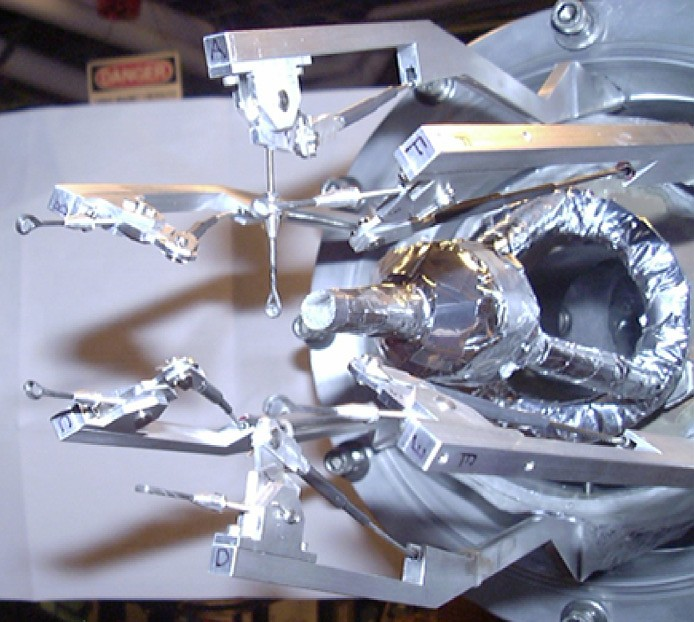
\includegraphics[width=7cm] {chap5-fig/PhTar.jpg} 
\caption {Picture of the {\it eg2} target system. The cryogenic target is 
in the back wrapped with aluminum foils, while solid targets are held by 
mechanical arms that were controlled remotely. In the picture, the top 
solid target is in the beam line.}
\label{fig:phototarget}
\end{figure}

The analysis of the experiment E-02-110, focusing on the study of color 
transparency effects, has been approved and published~\cite{ElFassi:2008}. As this 
analysis went through a careful review by the CLAS collaboration, we have 
adapted similar analysis methods as much as possible. In particular, the electron selection 
presented here is very similar to theirs; the main difference being a new 
target determination method. The pion identification cuts are, however, tightened
in this analysis as we have less constraints on the kinematics to exclude any possible pion contamination.

In the section \ref{sec:pid}, we identify the following particles, e$^-$, 
$\pi^-$ and $\pi^+$ using a series of cuts on various detector outputs. For 
pions, we require a signal in the drift chambers (DC) and scintillator counters (SC) in 
addition to the successful reconstruction of the time-based tracking. For electron 
identification, we use the same standards but requesting a good signal from 
all detectors, DC, Cherenkov Counters (CC), SC and Electromagnetic 
Calorimeter (EC).

Once all particles are identified, we extract our two observables, 
multiplicity ratios and the transverse momentum broadening. The derivation 
of these quantities is presented in section \ref{sec:obs}, while a list of 
corrections  is summarized in section \ref{sec:corrections}. The systematic 
uncertainty budget is detailed in section \ref{sec:TotSys}, and the final 
analysis results are presented and discussed in the next chapter.

\subsection{Particle Identification}
\label{sec:pid}

\subsubsection{Electron Identification}

First, we apply a fiducial cut on the EC local coordinates to remove electrons detected close to the calorimeter's edges ($U_{EC}>40$~cm, $V_{EC}<360$~cm and 
$W_{EC}<395$~cm). These hits are problematic because part of the electromagnetic shower might be generated outside of the detector. That leads to a wrong measurement of the energy deposited.

To reject pions, we apply a momentum-dependent cut of the energy deposited in the inner ($E_{in}$) and the outer parts ($E_{out})$ of the calorimeter as,

\begin{equation}
\label{einout}
\mu  \left[1-\frac{0.3}{\sqrt{a}}\right] - \frac{E_{in}}{p} \leq 
\frac{E_{out}}{p} \leq 
\mu  \left[1+\frac{0.3}{\sqrt{b}}\right] - \frac{E_{in}}{p},
\end{equation}

where $\mu = 0.271$ is the mean of the total energy fraction deposited in the 
calorimeter, the parameter $a$ is set to 0.5 and the parameter 
$b$ varies with momentum, as shown in table \ref{tab:ecoutin-par}. The derivation of $b$ was motivated by the non-linear momentum dependence of the energy 
deposited on both EC regions (see figure \ref{eleEC}). As pions are 
minimum ionizing particles, they are expected to loose a constant energy in 
the inner part of the calorimeter (around 30~MeV), regardless of their 
momenta. Therefore, by requesting more than 60~MeV to be deposited, we 
efficiently cut the pion contamination (see figure~\ref{eleECi}).

\begin{table}[tbp]
  \centering
  \begin{tabular}{@{} cc @{}}
    \hline
    Momentum bin (GeV/c)& Parameter b \\ 
    \hline
    0.5 - 0.7 & 0.85 \\
    0.7 - 0.9 & 0.8  \\
    0.9 - 1.1 & 0.85 \\
    1.1 - 1.3 & 1.05 \\
    1.3 - 1.5 & 1.1  \\
    1.5 - 1.7 & 1.35 \\
    1.7 - 1.9 & 1.35 \\
    1.9 - 2.1 & 1.45 \\
    2.1 - 2.3 & 1.35 \\
    2.3 - 2.5 & 1.35 \\
    2.5 - 2.7 & 1.35 \\
    2.7 - 2.9 & 1.3  \\
    2.9 - 3.1 & 1.35 \\
    3.1 - 3.3 & 1.35 \\
    3.3 - 3.5 & 1.5  \\
    3.5 - 3.7 & 1.6  \\
    3.7 - 3.9 & 1.8  \\
    3.9 - 4.1 & 1.8  \\
    4.1 - 4.3 & 1.8  \\
    4.3 - 4.5 & 1.8  \\
    \hline
  \end{tabular}
  \caption{Values of the parameter $b$ used in equation \ref{einout} for 
           different momentum ranges~\cite{ElFassi:2008}.}
  \label{tab:ecoutin-par}
\end{table}

\begin{figure}[p]
\centering
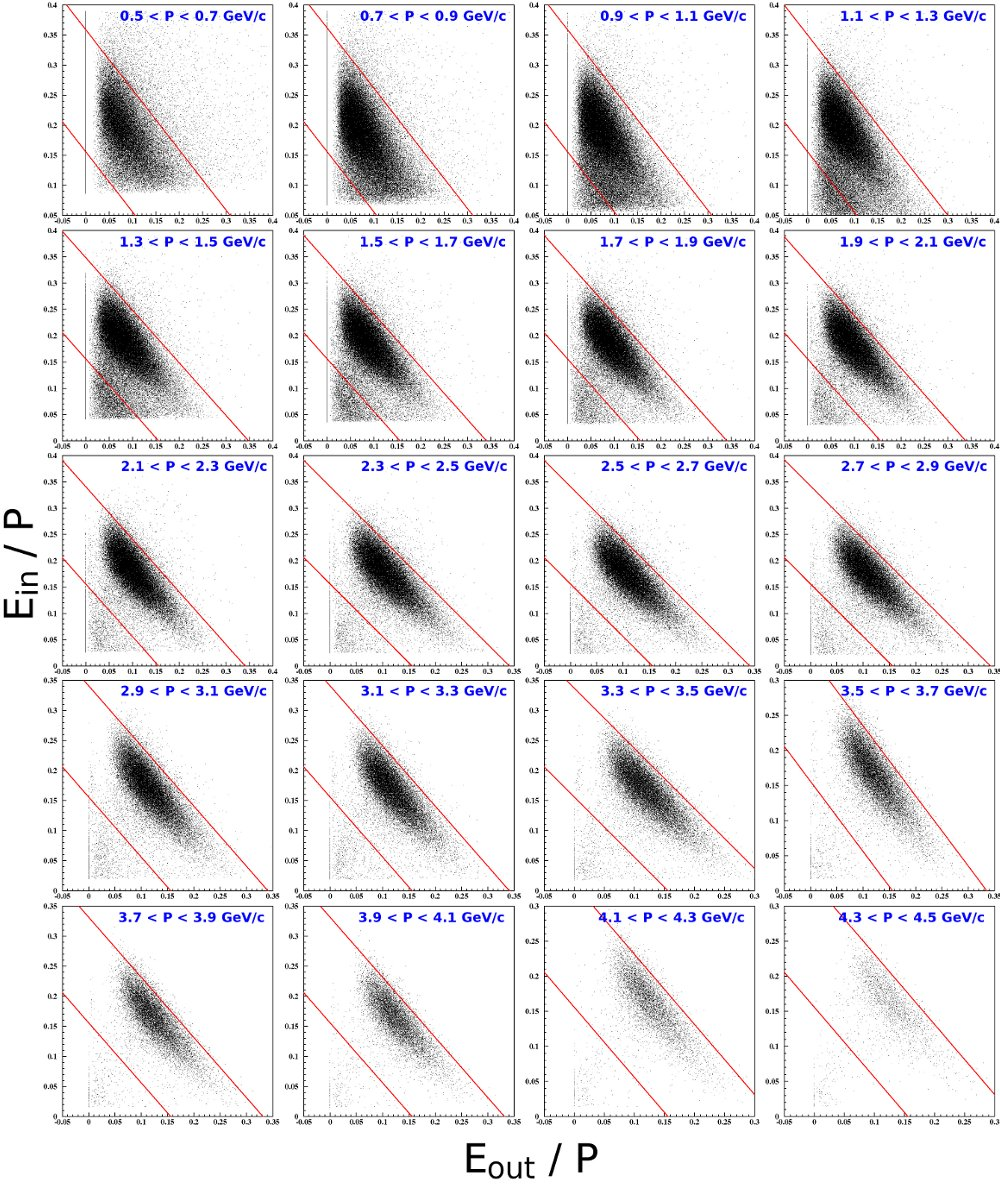
\includegraphics[width=14cm] {chap5-fig/fig02.jpg} 
\caption {Energy deposited in the inner part of the EC ($E_{in}$) as a function of the energy deposited in its outer part ($E_{out}$) normalized by tracks' momenta. Each panel is for a different momentum range, and the drawn red lines 
illustrate the cuts from equation \ref{einout}.}
\label{eleEC}
\end{figure}

\begin{figure}[tbp]
\centering
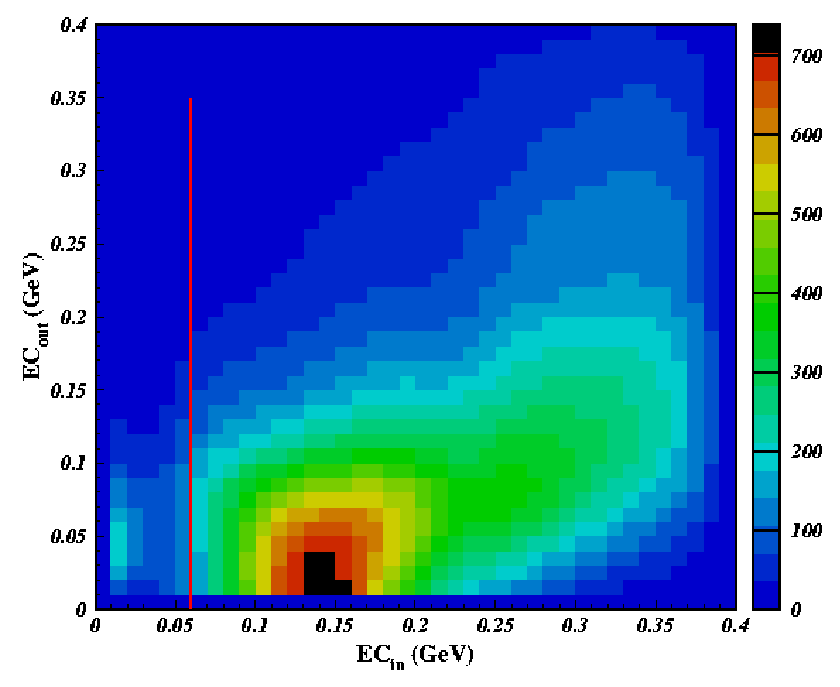
\includegraphics[width=9cm] {chap5-fig/fig03.png} 
\caption {Energy deposited in the inner part of the EC as a function of the 
energy deposited in its outer part. The red line illustrates the applied cut.}
\label{eleECi}
\end{figure}

In the CC, the mean number of photo-electrons\footnote{Photo-electrons are 
electrons produced in the front window of the Photo-Multiplier Tube (PMT) by the Cerenkov photons.} from a high energy electron is expected to be around 10.
However, hadrons can generate noise due to $\delta$ electrons produced in 
the materials of the detector. This signal is expected to be around 
one to two photo-electrons. Hence, to get rid of $\delta$-electrons, we kept only tracks with more than 2.5~photo-electrons, as depicted in figure \ref{delta}. 

\begin{figure}[tbp]
\centering
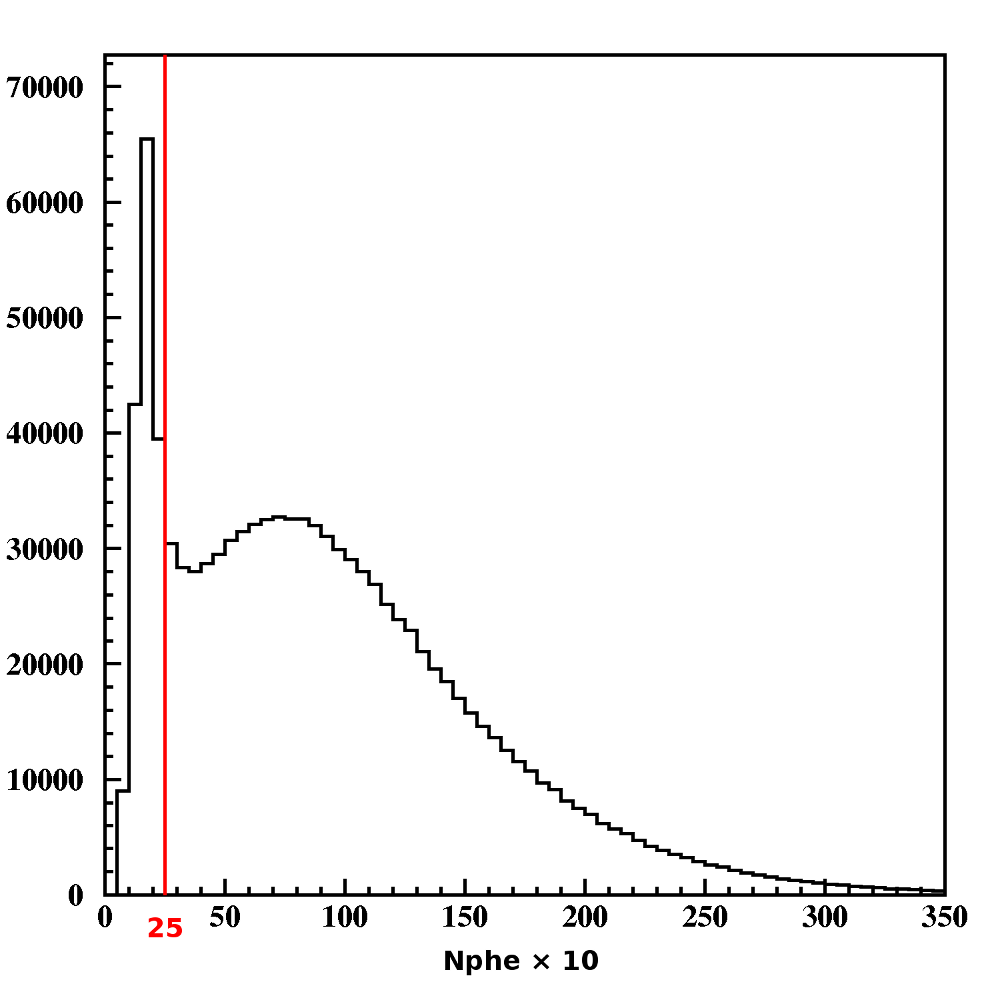
\includegraphics[width=8cm] {chap5-fig/fig04.png} 
\caption {Number of photo-electrons ($\times 10$) per tracks. The red line 
shows the applied cut to remove any low-energy pions' contamination.}
\label{delta}
\end{figure}

To select electrons, we also require that particles are negatively charged\footnote{In the CLAS reconstruction software, the electric charge is determined based on the tracks' bending direction in drift chambers.}.
Positively charged particles verifying electrons' cuts are identified as 
positrons. In the rest of this analysis, we used only events with a single electron and no positron to avoid any confusion between the scattered electron and electrons originating from hadronic decays or a photon conversion.

\subsubsection{$\pi^-$ Identification}
\label{PiId}

Pions are detected starting at a momentum of 250 MeV in the angular range 
from $\sim$10 to $\sim$140 degrees 
using only DC and SC signals. To identify negatively charged pions, we select 
negative tracks which were not identified as electrons already. 

This identification consists mostly of a time of flight (TOF) test. We define 
the relativistic particles' velocity difference as
$\Delta \beta = \beta_{measured} - {p \over \sqrt{p^2 + m_\pi^2}}$, which is required to be zero within $\pm 0.03$. Figure \ref{PionTOF} illustrates the effect of this cut. As we noticed there are not much negative kaons or anti-protons, we concluded that their contamination must be small (see section~\ref{SysId} for more detailed study).

The previous analysis from L. El Fassi et al. used $\pm 0.05$ ($\sim 3\sigma$), we decided
to reduce this number to about $2\sigma$ because of the difference of observables. The 
color transparency analysis was reconstructing the $\rho^0$ and implemented strong kinematical
cut that reduced significantly possible contaminations. Our measurement uses all the 
semi-inclusive production and is therefore more sensitive to contaminations. 

\begin{figure}[tbp]
\centering
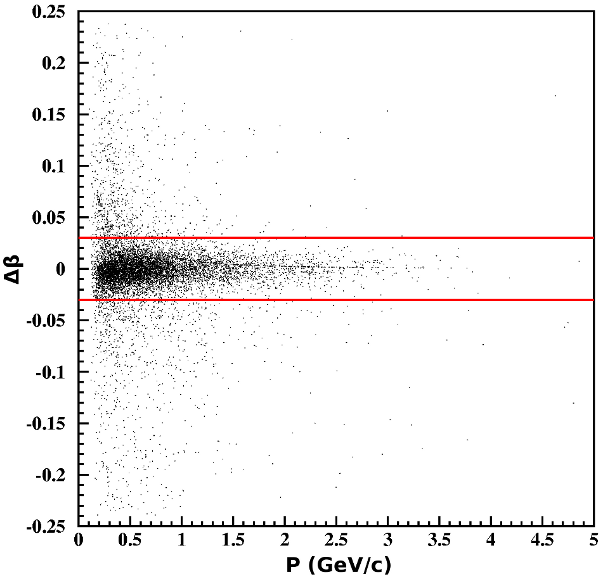
\includegraphics[width=8cm] {chap5-fig/fig05.png} 
\caption {$\Delta \beta$ of negatively charged particles as a function of momentum (GeV/c). The red lines shows the applied cuts to select negative pions.}
\label{PionTOF}
\end{figure}

In principle, a pion identification could be improved using the Cherenkov counter 
for momenta higher than 2.5~GeV/c. But, the observed low CC efficiency (see figure 
\ref{PionCC}) especially at momenta close to the CC threshold ($\sim$25\% at 
2.5~GeV/c and $\sim$50\% at 3~GeV/c) makes its use less compelling. 
Moreover, as only a very small amount of $K^-$s and no ${\bar p}s$ are present on figure \ref{PionTOF}, we decided to not use CC on this pions' identification.

\begin{figure}[tbp]
\centering
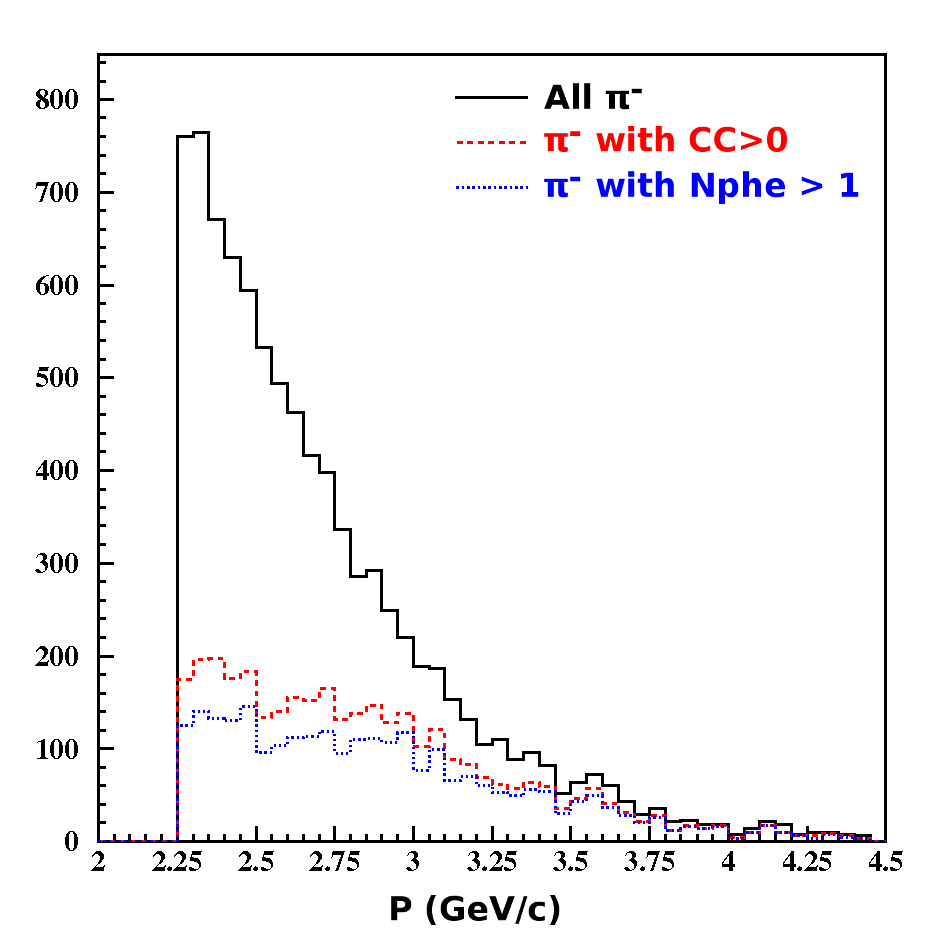
\includegraphics[width=8cm] {chap5-fig/fig06.png} 
\caption {Histograms of momentum (GeV/c) for $\pi^-$s. The black, red, and blue distributions are, respectively, for all identified $\pi^-$s, pions that fire Cherenkov counters, and pions that fire CC with more than one photo-electron.}
\label{PionCC}
\end{figure}

\subsubsection{$\pi^+$ Identification}

The identification of positively charged pions is similar to that of negative 
pions. However, the time of flight plot is significantly more busy (see figure 
\ref{PipTOF}), due to an important contamination from $K^+$s and protons at a
high momentum. As the CC is not efficient enough for a hadron separation, the 
kaons and protons contributions are reduced by the following tighter TOF cuts:

\begin{subequations}\label{TOF-Pip}
\begin{align}
    p_\pi &\leq 1.838 \text{ GeV/c : }
  & \Delta \beta &> \max\left(-0.03,{p \over\sqrt{p^2+0.4^2}}- {p \over \sqrt{p^2 + m_\pi^2}}\right), \\ 
    p_\pi &> 1.838    \text{ GeV/c : }
  & \Delta \beta &> \max\left(-0.02,{p \over\sqrt{p^2+0.7^2}}- {p \over \sqrt{p^2 + m_\pi^2}}\right).
\end{align}
\end{subequations}

\begin{figure}[tbp]
\centering
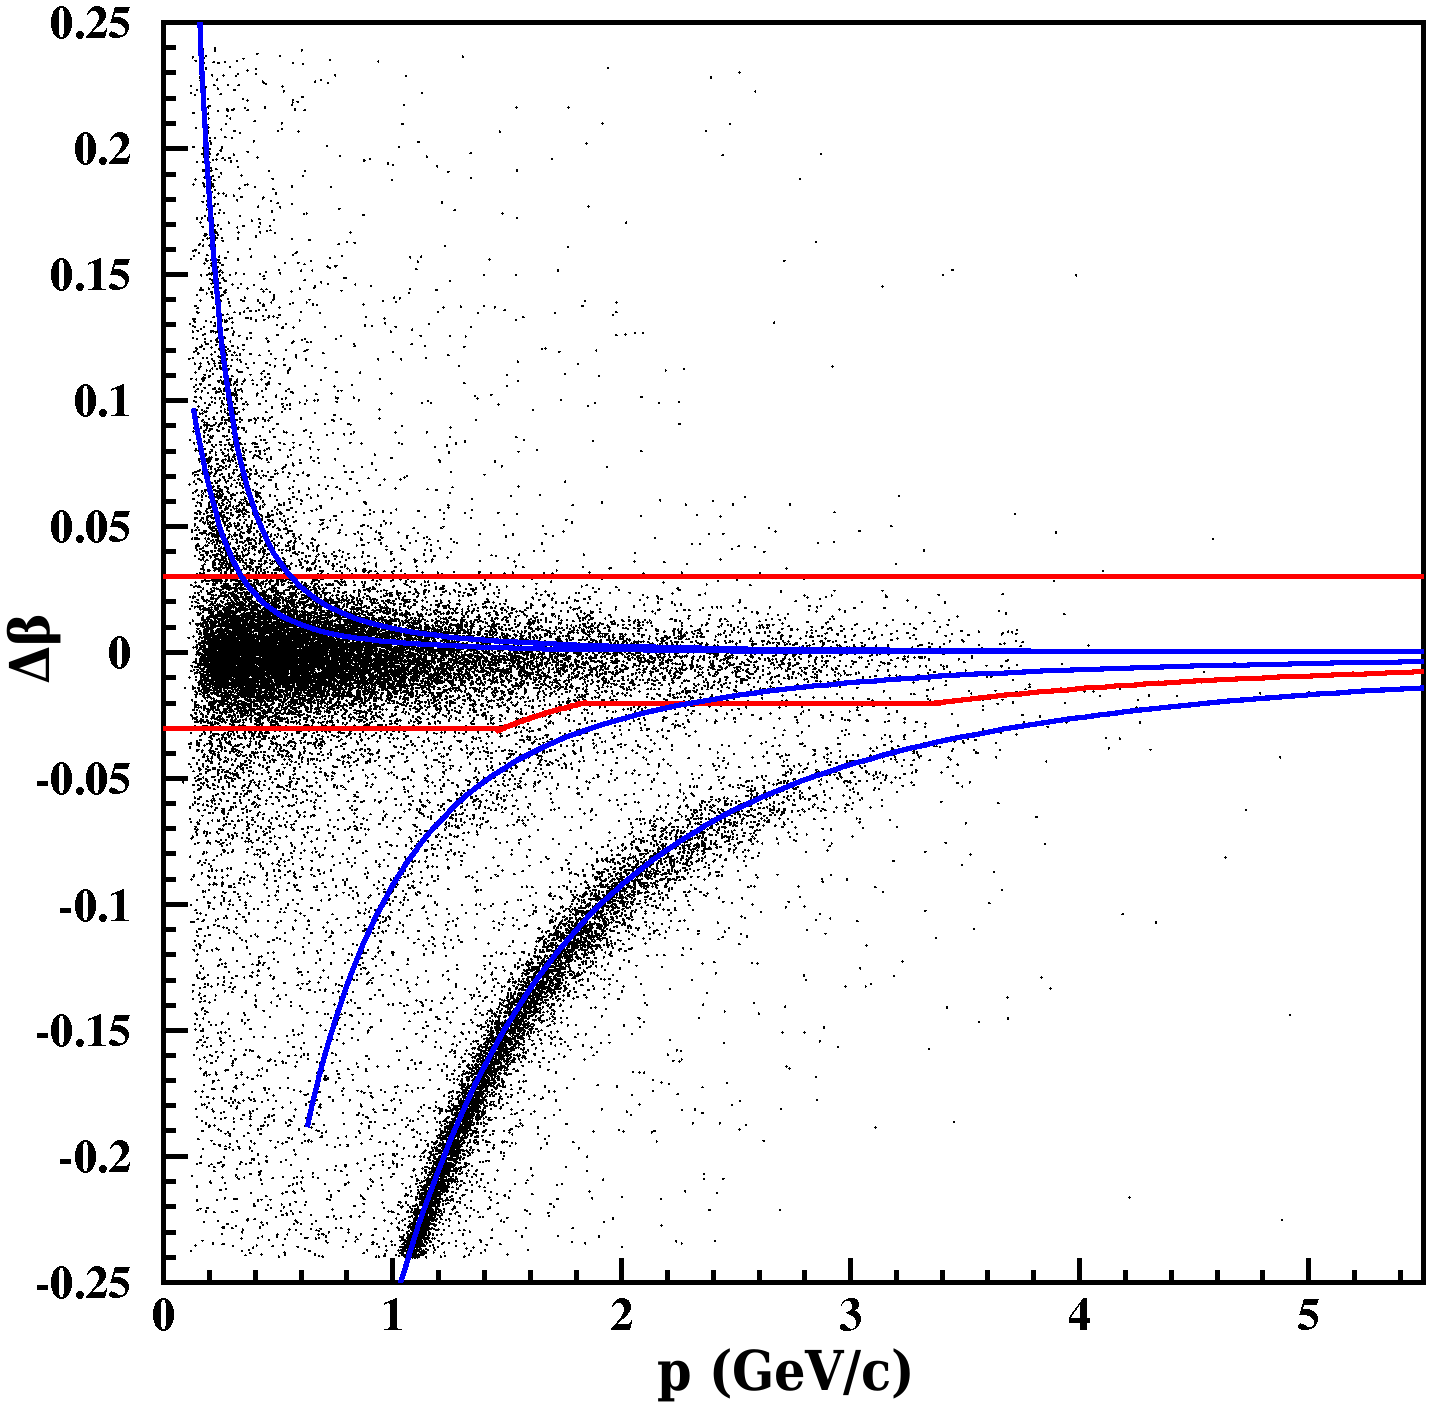
\includegraphics[width=8cm] {chap5-fig/pip_data.png} 
\caption {$\Delta \beta$ of positively charged particles as a function of momentum (GeV/c). The red lines shows the applied cuts to select positive pions. The blue lines indicate other particles' theoretical positions, and present from top to 
bottom positrons, muons, kaons and protons.}
\label{PipTOF}
\end{figure}

In opposition with negative pions, contamination sources are apparent and motivate a careful 
study of the TOF profile. One can see in figures~\ref{TOF-1}, \ref{TOF-2} and 
\ref{TOF-3} the $\Delta \beta$ profiles for many momentum slices. In figure~\ref{TOF-1}
one can see some contamination from lighter leptons ($e^+$ and $\mu^+$). These represent
a very small amount and one can see some justification for the choice of a $\pm 0.03$
cut as these particles do not appear to be discernable beyond that level. Similarly
in figure~\ref{TOF-2} one can see the contribution from kaons. The larger contribution
of this contamination motivated the tightening of the TOF cut on this side, to the limit
where kaons are a minority in the tail of the pion distribution. Finally a similar 
method is applied for the even larger proton contamination as shown in figure \ref{TOF-3}.

\begin{figure}[tbp]
\centering
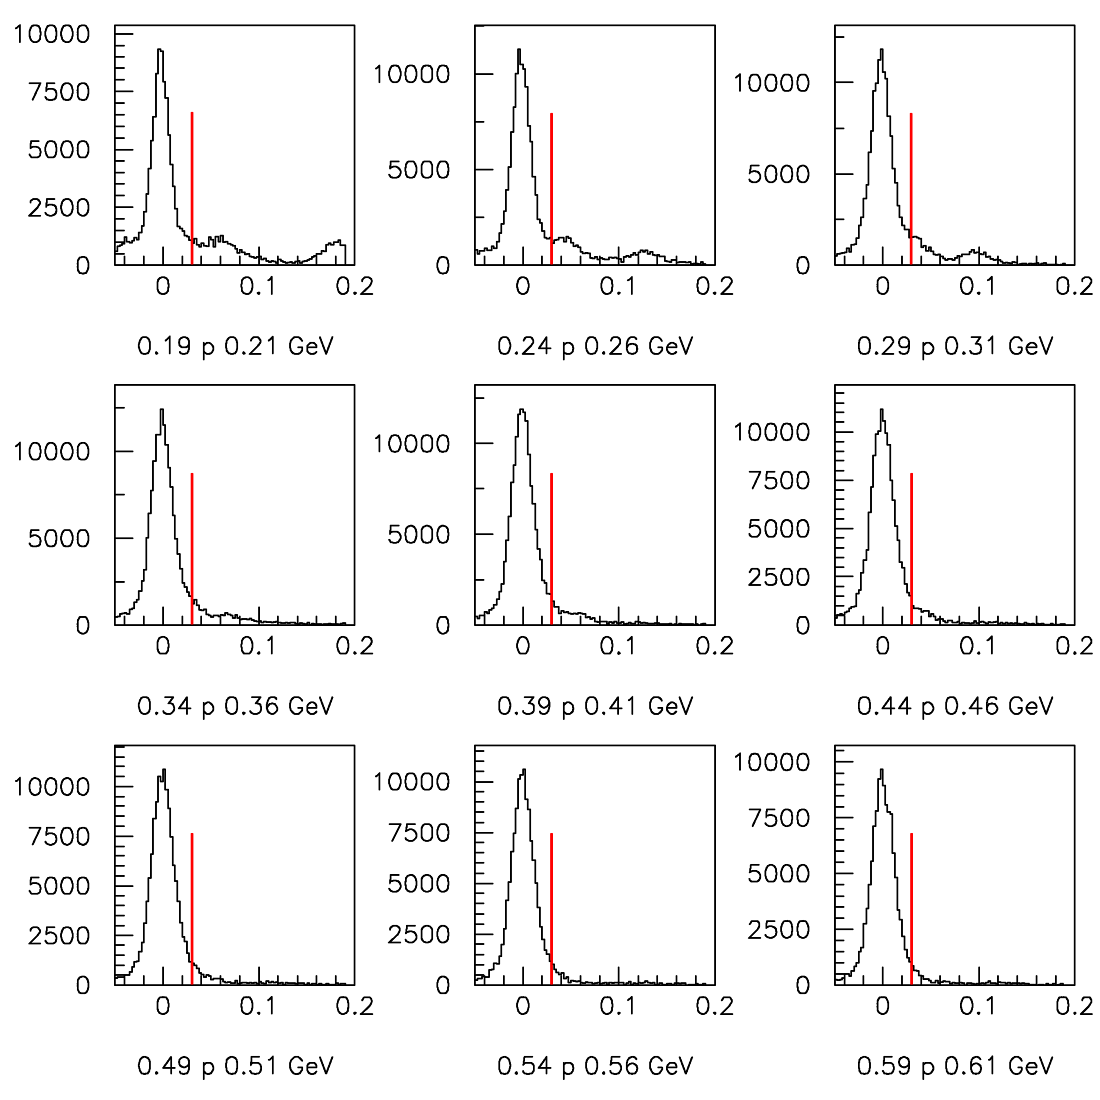
\includegraphics[width=8cm] {answer-fig/TofProfile1.png} 
\caption {$\Delta \beta$ of positively charged particles for low momentum slices 
(GeV/c). The red lines shows the applied cuts to select positive pions. The bumps on the right
correspond to muon and electron masses.}
\label{TOF-1}
\end{figure}

\begin{figure}[tbp]
\centering
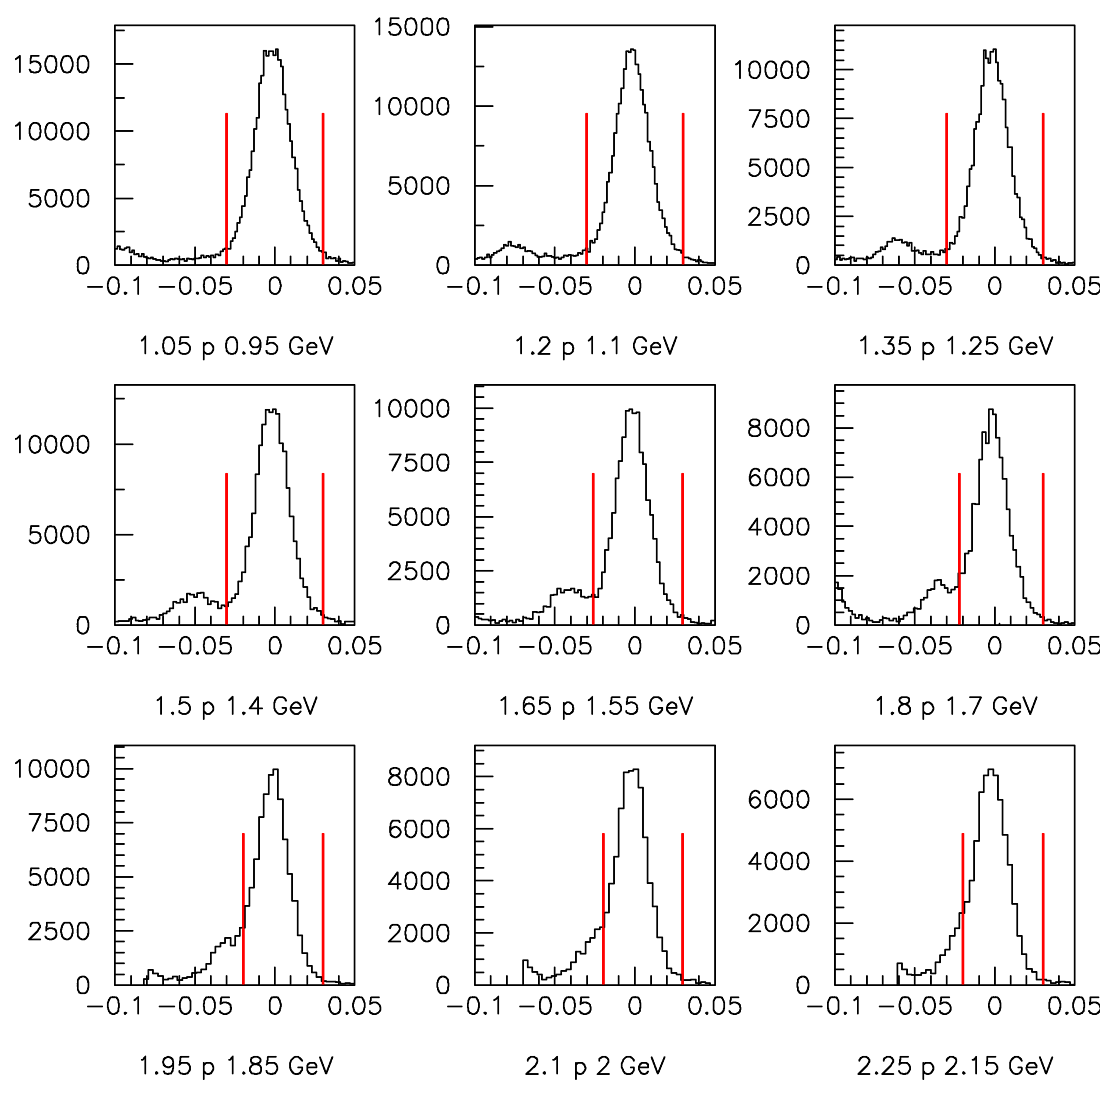
\includegraphics[width=8cm] {answer-fig/TofProfile2.png} 
\caption {$\Delta \beta$ of positively charged particles for medium momentum slices 
(GeV/c). The red lines shows the applied cuts to select positive pions. The bump on the left
correspond to the kaon mass.}
\label{TOF-2}
\end{figure}

\begin{figure}[tbp]
\centering
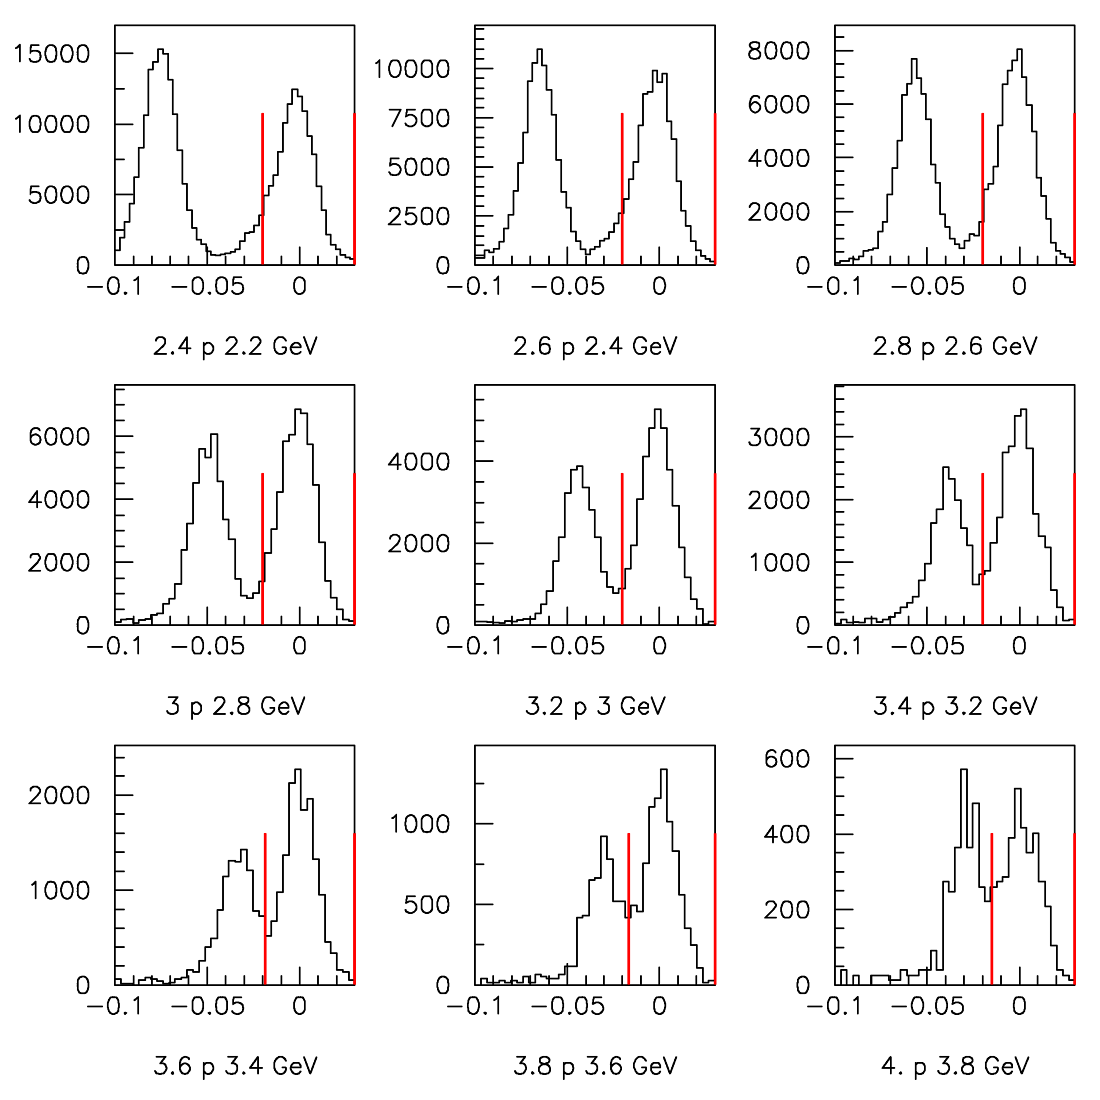
\includegraphics[width=8cm] {answer-fig/TofProfile3.png} 
\caption {$\Delta \beta$ of positively charged particles for high momentum slices 
(GeV/c). The red lines shows the applied cuts to select positive pions. The bump on the left
correspond to the proton mass.}
\label{TOF-3}
\end{figure}

These cuts minimize the kaon contamination, below 2.5~GeV/c, and the 
proton contamination for all momenta. The kaon contribution cannot be avoided, however, it should remain small (peaking $\sim$ 3\% according to our simulation) 
with only a small effect on our final results (see section \ref{SysId} 
for more details). Because protons could lead to even more contamination than kaons, 
a stricter cut is used at a high momentum. This cut is also justified by 
HERMES data \cite{Airapetian:2007vu}, which showed a very different behavior of protons compared to other hadrons.

\subsubsection{Target Determination}

To differentiate between the two targets and remove the background, we need to 
determine the point of origin of our final-state particles. As illustrated in figure~\ref{vertex}, the small misalignment of the beam with the CLAS detector led to an artificial shift on different sectors' z-vertex positions. To correct from this effect, we added the shift shown in table~\ref{tab:vertex} when determining each particle's vertex position. Those values were obtained from the fit of the solid target distribution on each sector.

\begin{figure}[p]
\centering
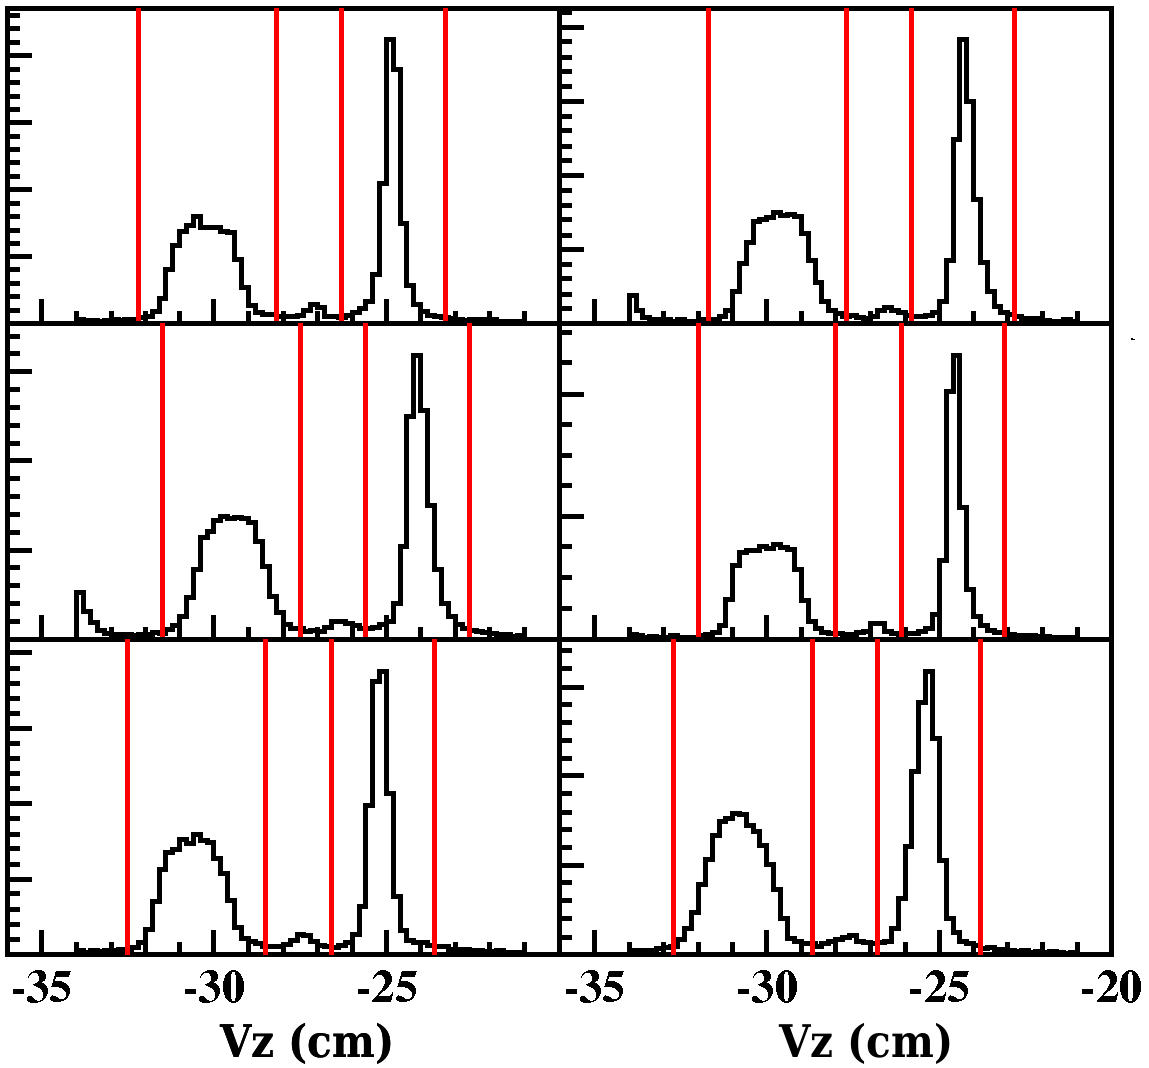
\includegraphics[width=10cm] {chap5-fig/Vertex_el_data.png}
\caption {Sector-by-sector electrons' vertex distributions. The latter are reconstructed along the beam direction and relative to the center of CLAS located at 0~cm. The red lines show the applied cuts to select the two targets.}
\label{vertex}
\end{figure}

\begin{table}[p]
  \centering
  \begin{tabular}{@{} cc @{}}
    \hline
    Sector & Shift (cm) \\ 
    \hline
    1 & + 0.1 \\ 
    2 & - 0.4 \\ 
    3 & - 0.6 \\ 
    4 & - 0.1 \\ 
    5 & + 0.4 \\ 
    6 & + 0.6 \\ 
    \hline
  \end{tabular}
  \caption{Values used to correct the vertex position on each sector}
  \label{tab:vertex}
\end{table}

The detected electrons are associated with the solid target if their vertex 
position is less than 1.5~cm ($\sim$3~$\sigma$) from the values shown on table 
\ref{tab:targets}. For the liquid target, the cut is a bit larger, 2 cm, in order to count for the cryogenic target's size (see figure \ref{vertex}). The pions' vertex was checked against the electron one and was imposed to satisfy this additional condition $| Vz^{e^-} - Vz^{\pi} | < 3$ cm (see figure \ref{fig:dvzpi}).

\begin{figure}[tbp]
\centering
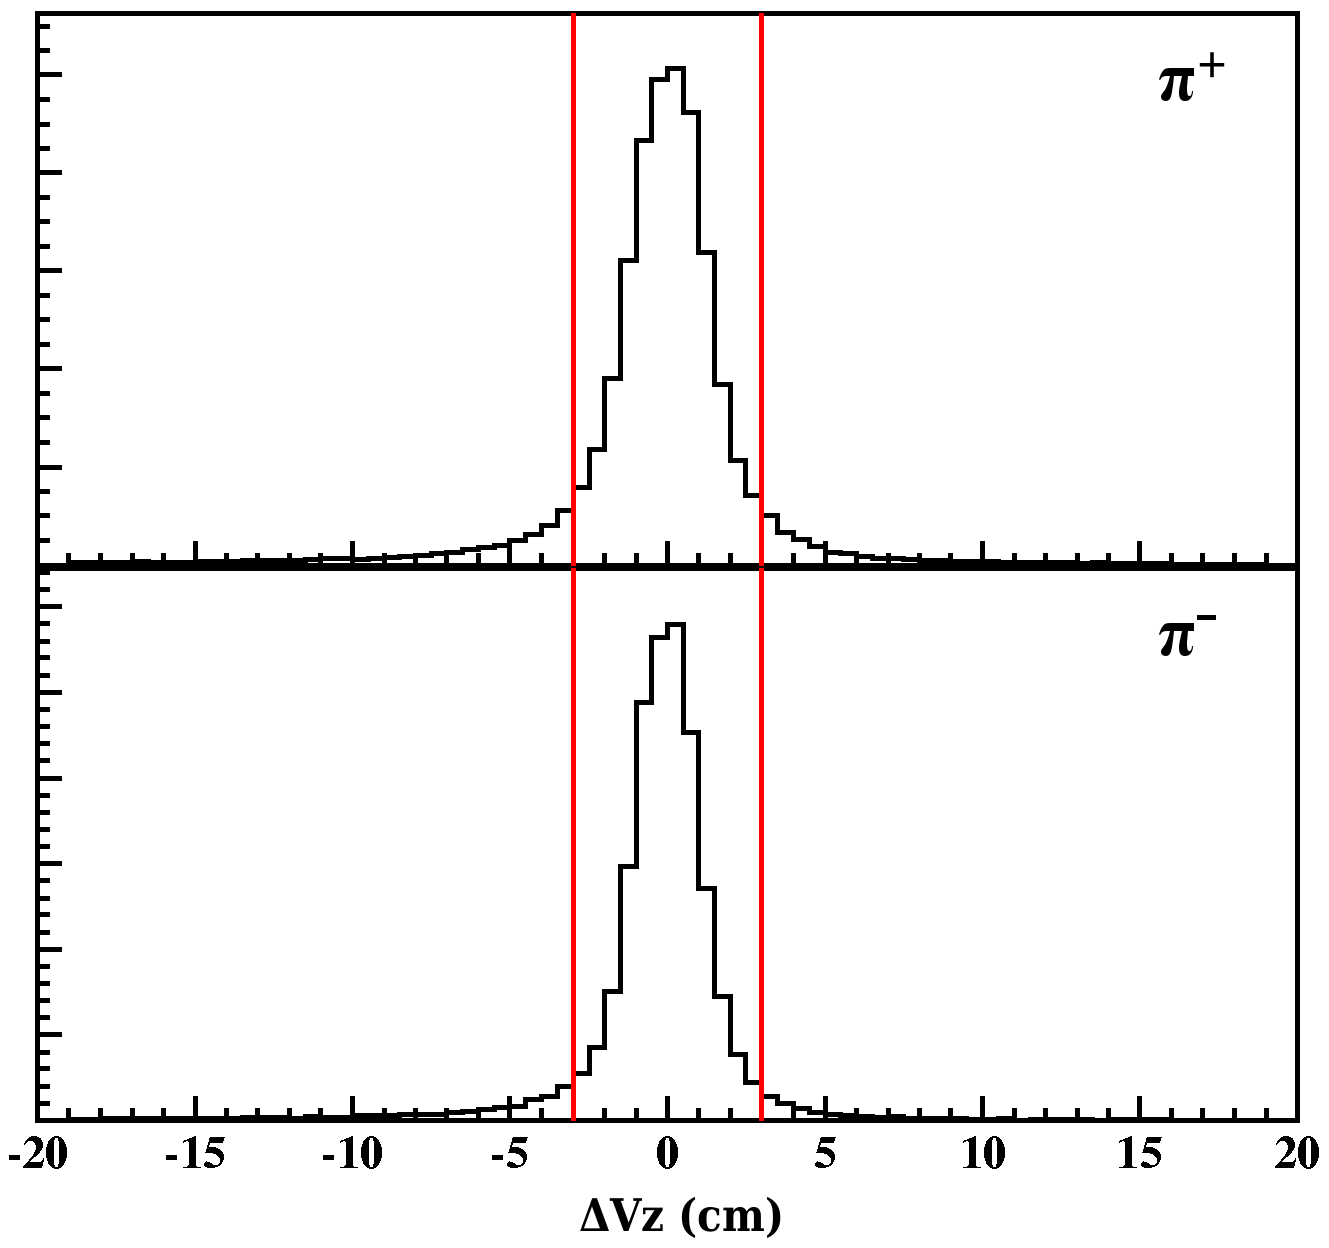
\includegraphics[width=8cm] {chap5-fig/Vertex_pi_data.png}
\caption {The difference between electrons and pions z-vertex positions. $\pi^+$s and $\pi^-$ are plotted, respectively, in the top and bottom panels. The red lines show the applied cuts to select both pions.}
\label{fig:dvzpi}
\end{figure}

The position of our targets could also vary from a run to another, but this was not significant in this experiment. Indeed, except for aluminum, other targets remained in the same position within one or two millimeters. All targets' positions, in CLAS coordinates, are given in table \ref{tab:targets}. 
We show in figures \ref{VertexSolid} and \ref{VertexLiquid} the evolution 
of the position of the targets with run number. The data where the aluminum
target is off by 1 cm has been excluded from the analysis. Other variations
appear to be of a mm or less, while the gap between the solid and liquid target
is about 5 cm. They should therefore have negligible contribution to the 
error on acceptance corrections in regard to the error budget already associated
to the measurements.

\begin{table}[p]
  \centering
  \begin{tabular}{|c|c|c|c|c|c|c|}
    \hline
    Target & Carbon & Al (1) & Al (2) & Iron   & Tin    & Lead   \\ 
    \hline \hline
    Liquid & -30.1  & n/a    & n/a    & -30.2  & -30.1  & -30.1  \\ 
    Solid  & -24.7  & -25.0  & -23.8  & -24.9  & -23.8  & -24.9  \\
    \hline
  \end{tabular}
  \caption{The measured mean vertex position of our nuclear targets relative to the center of CLAS (in cm). Must note that aluminum data are separated in two sets because this target's position has brutally changed. Moreover, during these runs the deuterium target was empty.}
  \label{tab:targets}
\end{table}

\begin{figure}[tbp]
\centering
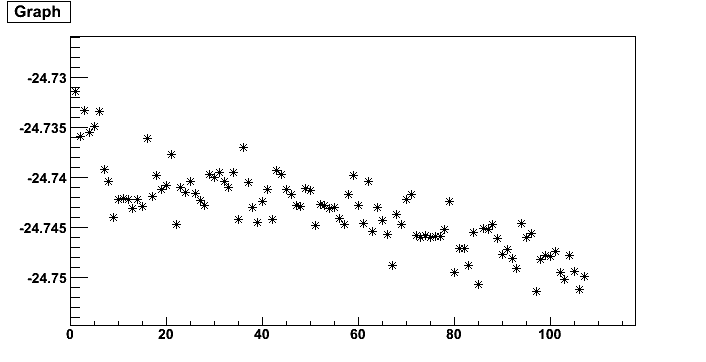
\includegraphics[width=7.5cm] {answer-fig/VertexC.png} 
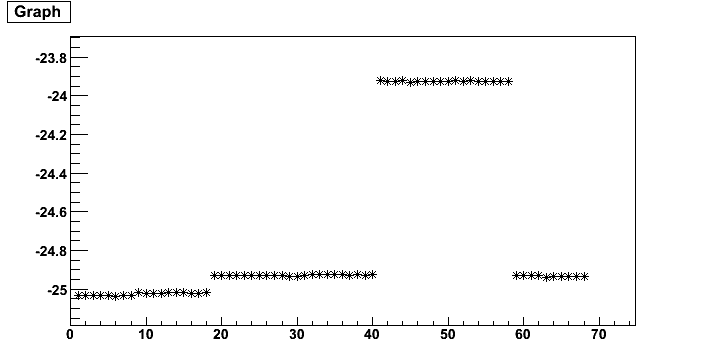
\includegraphics[width=7.5cm] {answer-fig/VertexAl.png} 
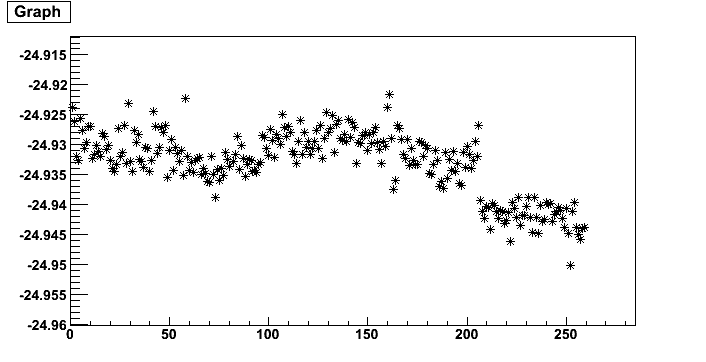
\includegraphics[width=7.5cm] {answer-fig/VertexFe.png} 
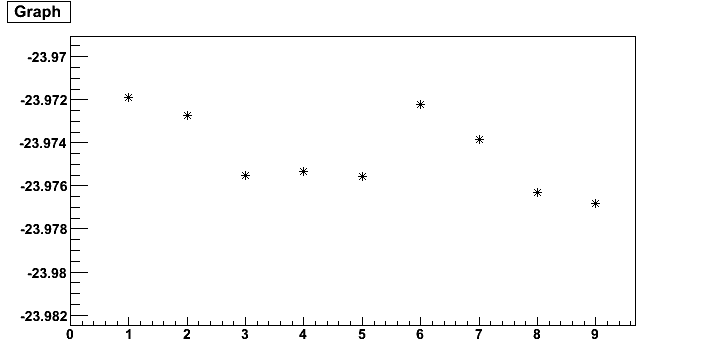
\includegraphics[width=7.5cm] {answer-fig/VertexSn.png} 
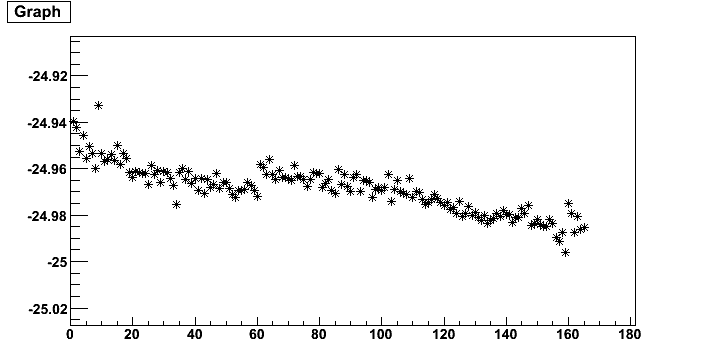
\includegraphics[width=7.5cm] {answer-fig/VertexPb.png} 
\caption {Vertex origin along $z$ (in cm) of electrons as a function of run 
number for the different solid targets. Top left is for carbon, top right
aluminum, middle left iron, middle right tin and bottom is for lead.}
\label{VertexSolid}
\end{figure}

\begin{figure}[tbp]
\centering
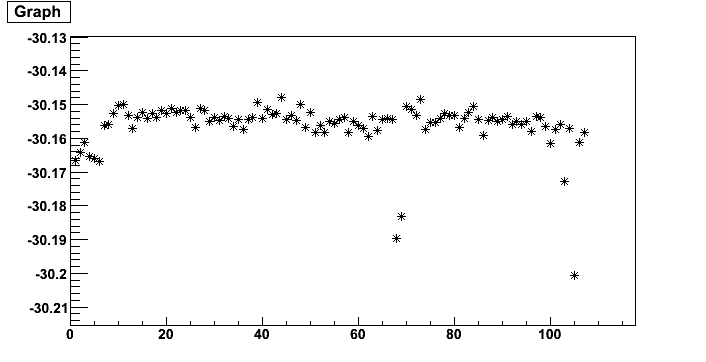
\includegraphics[width=7.5cm] {answer-fig/VertexDeutC.png} 
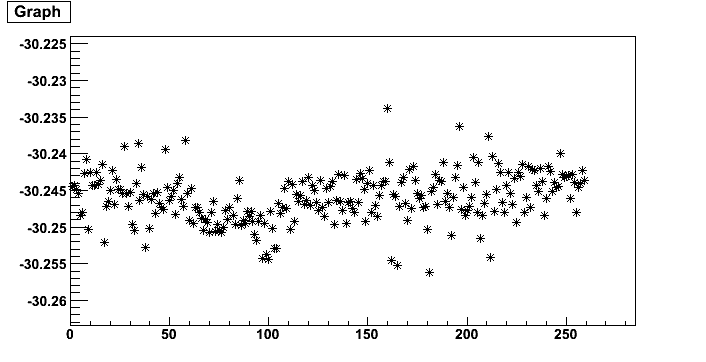
\includegraphics[width=7.5cm] {answer-fig/VertexDeutFe.png} 
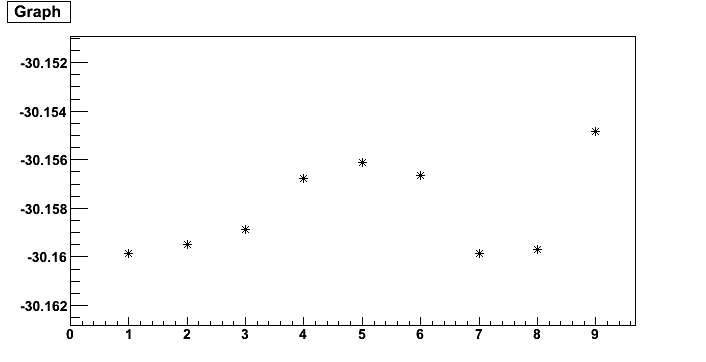
\includegraphics[width=7.5cm] {answer-fig/VertexDeutSn.png} 
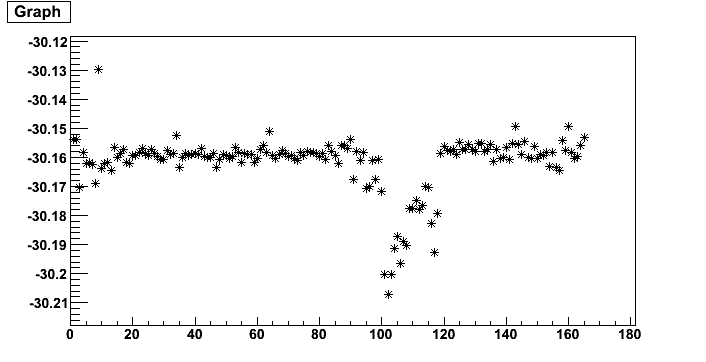
\includegraphics[width=7.5cm] {answer-fig/VertexDeutPb.png} 
\caption {Vertex origin along $z$ (in cm) of electrons as a function of run 
number for the deuterium target in different solid targets configurations.
Top left is for carbon, top right iron, bottom left tin and bottom right is for lead.}
\label{VertexLiquid}
\end{figure}

\subsubsection{Data Quality}

To check the quality of the runs\footnote{Runs are typically stopped every two hours
of data taking, but they can be smaller when experimental problems arrise.}, we 
monitored the ratio of scattered electrons yields obtained from solid and liquid 
targets. In case of the beam hitting other materials in the beam-line or of any 
other problems that would affect our final result, 
this ratio will be off and indicate the problematic runs. In figure 
\ref{DataQ}, we show the electron yield ratios for different nuclear target; we 
fitted these ratios to determine the mean value for each target, then we discarded 
runs that were 5~$\sigma$ away from the appropriate mean. Must note that these 
ratios were consistent with our target's thicknesses given in \cite{Hakobyan:2008zz} 
except for the carbon target. For that reason, the density of the latter was 
remeasured, and its new value was finally matching our 
data\footnote{i.e. (1.747+/-0.0007)g/cm$^3$ instead of 2.235 g/cm$^3$}.

\begin{figure}[tbp]
\centering
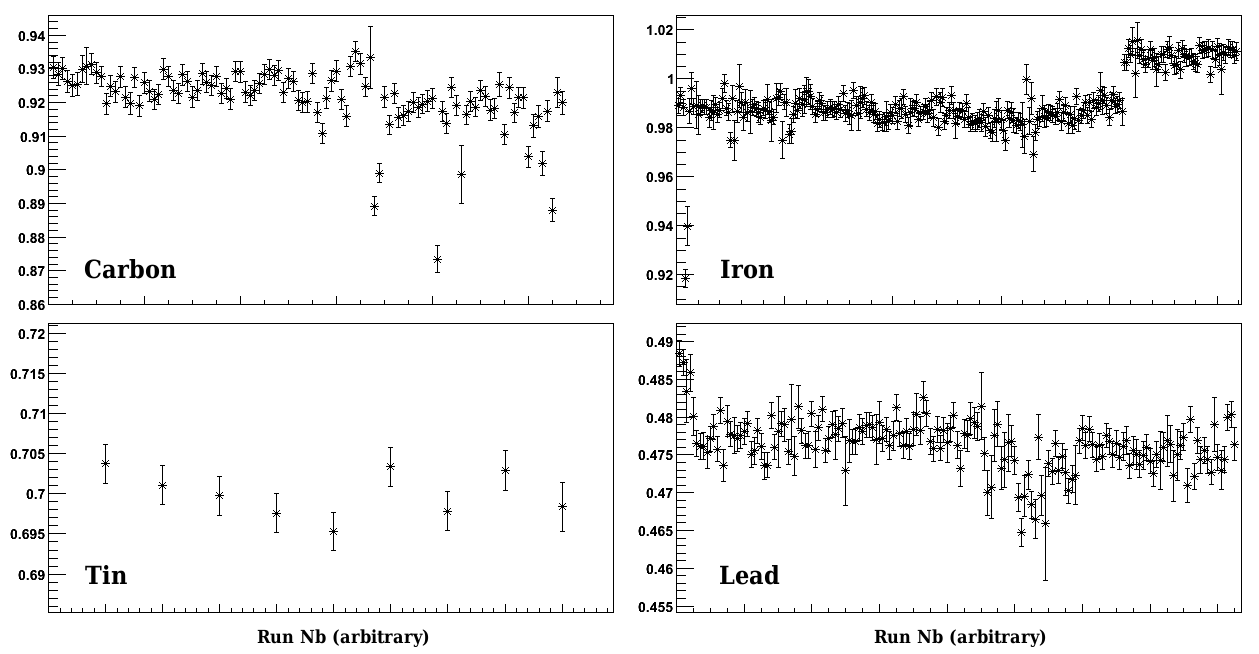
\includegraphics[width=15cm] {chap5-fig/TargetElRatio.png}
\caption {Ratio of scattered electrons yields (solid over deuterium) for each run.}
\label{DataQ}
\end{figure}

%TODO provide an updated target table

\subsection{Extraction of Multiplicity Ratio and $\Delta$P$_\perp^2$}
\label{sec:obs}

Since we are interested in deep inelastic scattering, we use the following 
cuts: $Q^2 > 1$~GeV$^2$/c$^2$ and $W > 2$~GeV/c$^2$, with the inclusive distributions
after these cuts shown in figure \ref{DISKine}.

\begin{figure}[tbp]
\centering
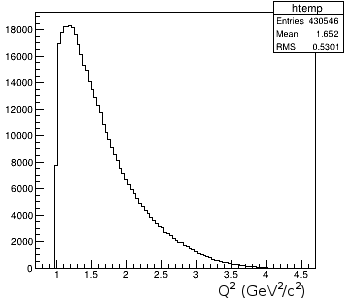
\includegraphics[width=5cm] {answer-fig/DIS-Q2.png} 
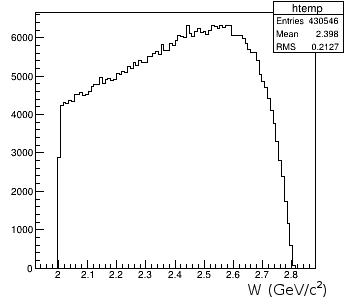
\includegraphics[width=5cm] {answer-fig/DIS-w.png} 
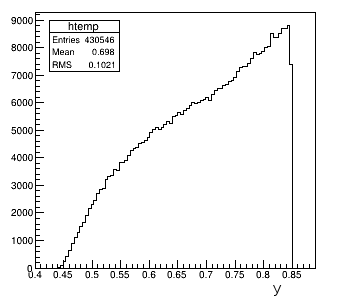
\includegraphics[width=5cm] {answer-fig/DIS-y.png} 
\caption {Inclusive distributions after DIS selection cuts for a sample of the iron
data.}
\label{DISKine}
\end{figure}

We also apply a cut on the energy transferred fraction, $y = \nu/E_{beam} < 0.85$. This cut aims to remove the low energy electrons that are significantly affected by radiative effects and are at the limit of our trigger threshold.

\subsubsection{Method}
\label{RatioCalc}

Once the identification is done, the calculation of our two observables and their statistical uncertainties is straightforward. The latter are given by:
\begin{equation}
\label{eq:MRError}
{\delta \left ( R_A^h \right ) \over R_A^h} = \sqrt{ 1 /N_A^h + 1/ N_A^e +1/N_D^h + 1/N_D^e}
\end{equation}
and
\begin{equation}
\label{eq:DPtError}
\left ( \delta \left ( \Delta \langle P_\perp^2 \rangle \right ) \right )^2 = 
   \left ({\langle P_\perp^4 \rangle - \langle P_\perp^2 \rangle ^2}\right )_A / N_A^h
 + \left ({\langle P_\perp^4 \rangle - \langle P_\perp^2 \rangle ^2}\right )_D / N_D^h.
\end{equation}

However, the implementation of acceptance and radiative corrections is done through weights associated to each event based on its kinematics. The multiplicity ratio then becomes
\begin{equation}
R_A^h (Q^2,\nu,z_h,P_\perp^2) = {{\sum \omega_A^h (Q^2,\nu,z_h,P_\perp^2) / \sum \omega_A^e (Q^2,\nu)} 
                       \over {\sum \omega_D^h (Q^2,\nu,z_h,P_\perp^2) / \sum \omega_D^e (Q^2,\nu)}},
\end{equation}
where the sums run over all the events and $\omega$ is the weight associated with the event. The expression of the transverse momentum broadening remains as
\begin{equation}
\Delta \langle P_\perp^2 \rangle = \langle P_\perp^2 \rangle_A - \langle P_\perp^2 \rangle_D,
\end{equation}
but with
\begin{equation}
\langle P_\perp^2 \rangle = {\sum \left ( P_\perp^2 \times \omega (Q^2,\nu,z_h,P_\perp^2) \right ) \over \sum \omega (Q^2,\nu,z_h,P_\perp^2)}.
\end{equation}

Thus, new expressions of the weighted statistical uncertainties are derived: 
\begin{equation}
{\delta \left ( R_A^h \right ) \over R_A^h} = 
      \sqrt{ \left ( {\sum {\omega^h_A}^2 \over \left (\sum \omega^h_A \right )^2} \right ) 
           + \left ( {\sum {\omega^e_A}^2 \over \left (\sum \omega^e_A \right )^2} \right ) 
           + \left ( {\sum {\omega^h_D}^2 \over \left (\sum \omega^h_D \right )^2} \right ) 
           + \left ( {\sum {\omega^e_D}^2 \over \left (\sum \omega^e_D \right )^2} \right ) }
\end{equation}
 and 
\begin{equation}
\begin{split}
\left ( \delta \left ( \Delta \langle P_\perp^2 \rangle \right ) \right )^2 = 
   \left ({{\sum \omega^h_A P_\perp^4 }\over{\sum \omega^h_A}} 
 - \left ({\sum \omega^h_A P_\perp^2 }\over{\sum \omega^h_A}\right )^2 \right ) 
         \times \left ( {\sum \left ( {\omega^h_A}^2 \right ) \over 
                \left ( \sum \omega^h_A \right ) ^2 }\right ) \\
 + \left ({{\sum \omega^h_D P_\perp^4 }\over{\sum \omega^h_D}} 
 - \left ({\sum \omega^h_D P_\perp^2 }\over{\sum \omega^h_D}\right )^2 \right ) 
	 \times \left ( {\sum \left ( {\omega^h_D}^2 \right ) 
          \over \left ( \sum \omega^h_D \right ) ^2 }\right ).
\end{split}
\end{equation}

Following the first round of questions from the analysis review committee, we
reflected about this implementation of error bars and possible overlap with the 
systematic errors evaluated below. First we found an error with how the formula
for transverse momentum broadening was implemented and corrected it. This 
reduces the size of statistical 
error bars of the transverse momentum broadening by roughly a factor 2 to 3. 
We also reflected that the correlation between the weights should reduce
the statistical errors. In a given bin the weights associated with each 
targets are always of similar sizes, this correlation will reduce the size of 
error bars. However, we do not see a method to properly take this 
effect fully into account in term of purely statistical error bars, and
remains as is. Finally, 
it was noted that some of the effects were double counted once through the 
statistical error on the acceptance correction and the systematics associated
with the correction. So, we decided to account only the systematic error budget
and use purely statistical errors of equations
\ref{eq:MRError} and \ref{eq:DPtError}. In summary, we concluded that the 
systematic error contribution associated to the statistics of the 
simulation sample were indeed a double counting and are not used anymore
in any error bars.

\subsubsection{Preliminary Results}
\label{prelim}

To provide some insight into the quality of our data, we present in 
figure~\ref{fig:prelim} a few preliminary results before the application of 
any corrections. These preliminary results will be used also to illustrate 
the effects of the corrections discussed below.

\begin{figure}[htb]
\centering
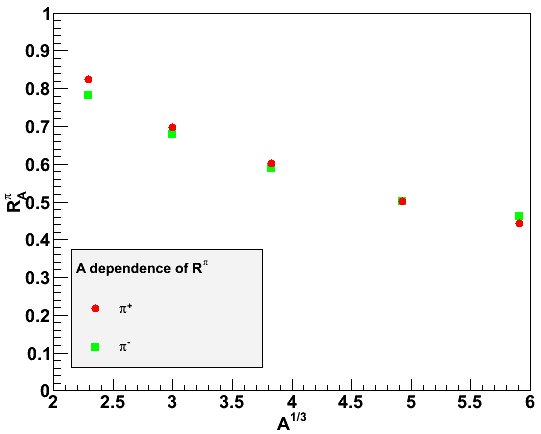
\includegraphics[width=7.4cm] {chap5-fig/a_RvA.png} 
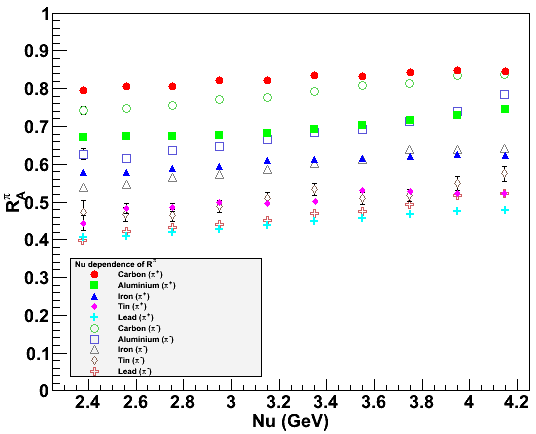
\includegraphics[width=7.4cm] {chap5-fig/a_RvZ.png} 
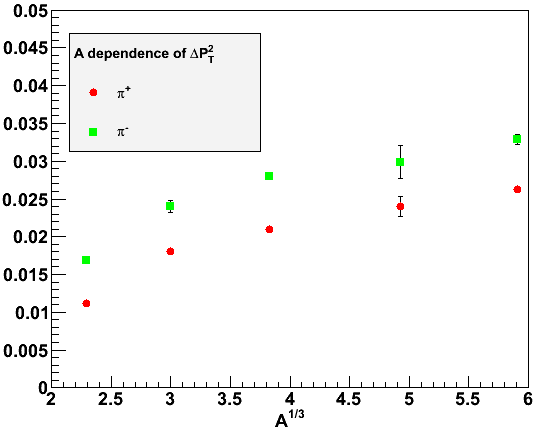
\includegraphics[width=7.4cm] {chap5-fig/a_PvA.png} 
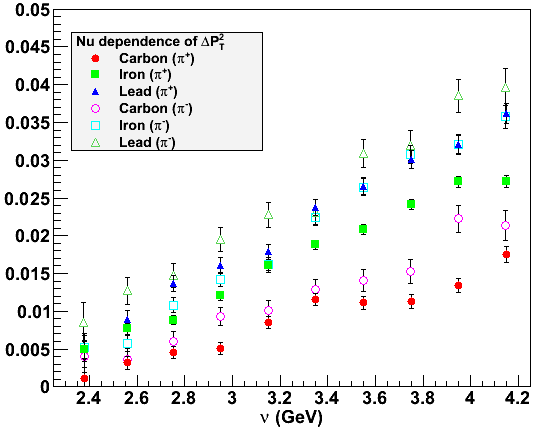
\includegraphics[width=7.4cm] {chap5-fig/a_PvNu.png} 
\caption {Results for multiplicity ratios (top) and the transverse momentum 
broadening (bottom) before applying any corrections.}
\label{fig:prelim}
\end{figure}


\subsection{Corrections}
\label{sec:corrections}

\subsubsection{Acceptance Correction}
\label{sec:accept}

The acceptance correction consists of applying weights to the experimental data
event by event to correct for any detection inefficiencies of used detectors.
Incidentally, it also corrects for other small detection issues, such as 
misidentification and re-scattering on detector material. The quality 
of the correction depends on the ability of the simulation to reproduce the 
experiment, the accumulated statistics, and the size of interfering effects, such 
as the bin migration. For this correction, we applied the method from the 
approved and published analysis from the same eg2 data~\cite{ElFassi:2008}.

\paragraph{Simulation} ~\\
To correct for acceptance effects, we simulated a total of 100 million events 
per target ($^2$H, C, Fe and Pb) using the PYTHIA \cite{Sjostrand:2006za} 
event generator that was slightly modified to include Fermi motion effects. The 
generated events are processed by CLAS softwares (GSIM, GPP and user\_ana) 
to simulate the detector and the reconstruction process in a fashion similar 
to that done with the experimental data.
% TODO GPP factors

The simulated data are processed like the experimental data by 
applying the cuts described in the section \ref{sec:pid}. Overall the 
simulation reproduces quite well the detector response, yet two issues might 
affect us and have to be understood. First, the efficiency of the CC is 
overestimated in the simulation. On the electron side the signal is a little stronger in the simulation (11 
photo-electrons) compared to experimental data (8 photo-electrons), but this 
feature should not affect us too much, because we are cutting only the tail of the 
distribution in both cases. Second, since in the simulation the beam is perfectly aligned with CLAS, the vertex cuts do not need to be shifted from one sector to an other. Therefore, we do not apply the shift from table \ref{tab:vertex} to the simulated data; the resulting cuts are shown in figure~\ref{simvertex}.

\begin{figure}[tpb]
\centering
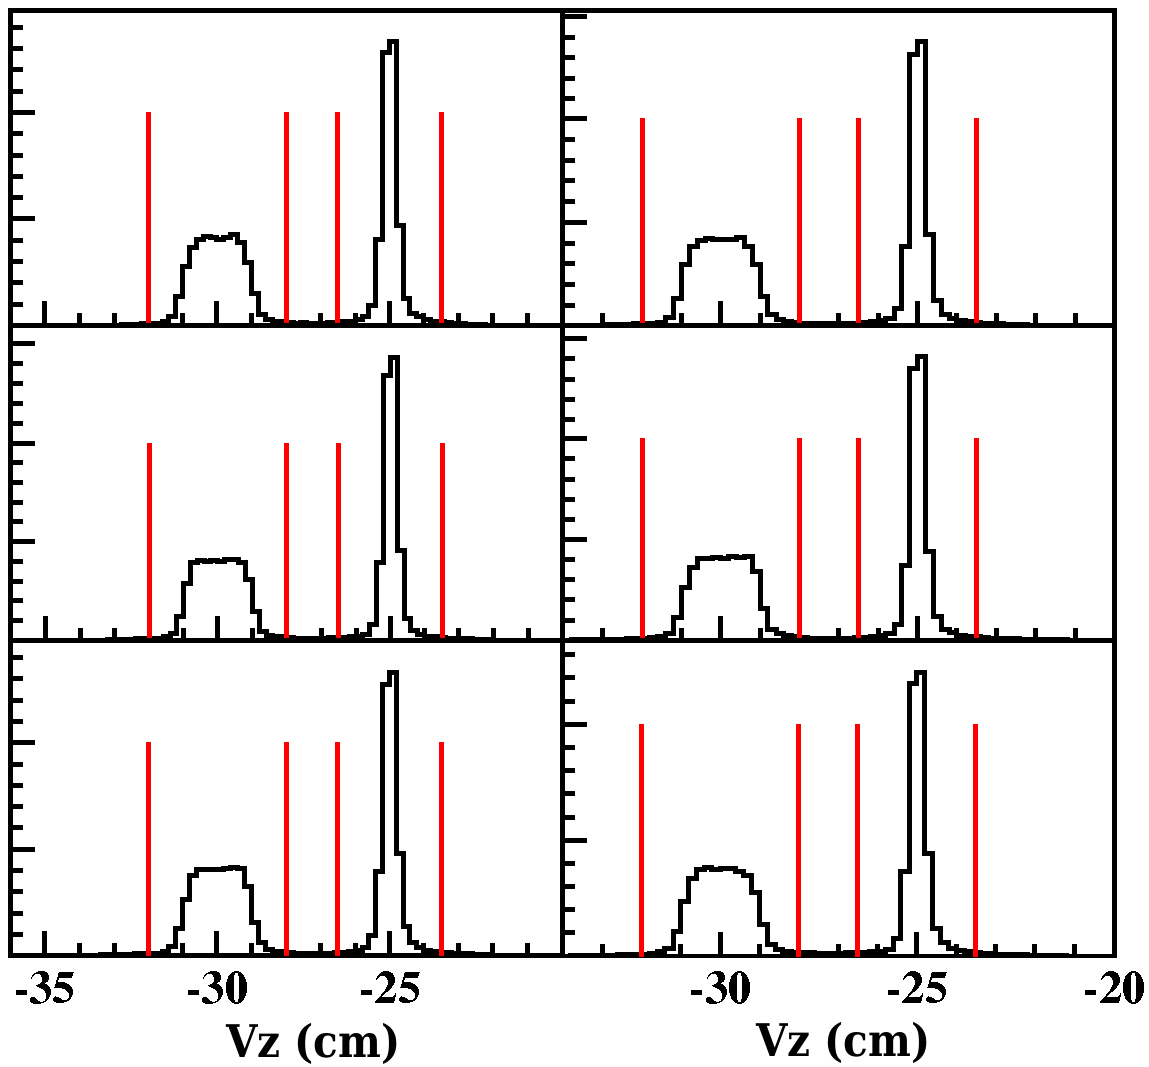
\includegraphics[width=9cm] {chap5-fig/Vertex_el_sim.png}
\caption {Sector by sector electrons' vertex distributions from the {\bf simulated data}. The latter are reconstructed along the beam direction, and relative to the CLAS center. The red lines show the used cuts to select both targets.}
\label{simvertex}
\end{figure}

The kinematical distributions from the simulation are compared to the 
experimental ones. This is important for the acceptance correction, to see 
whether or not, we can integrate over any variables in this correction.
Comparisons between simulated and experimental data are shown in figures 
\ref{fig:compNuQ2} to \ref{fig:compPhih}. The agreement is reasonable, but not 
perfect. The differences are due to the PYTHIA simulation, which is not including some 
physical effects, such as radiative and diffractive processes.

\begin{figure}[tbp]
\centering
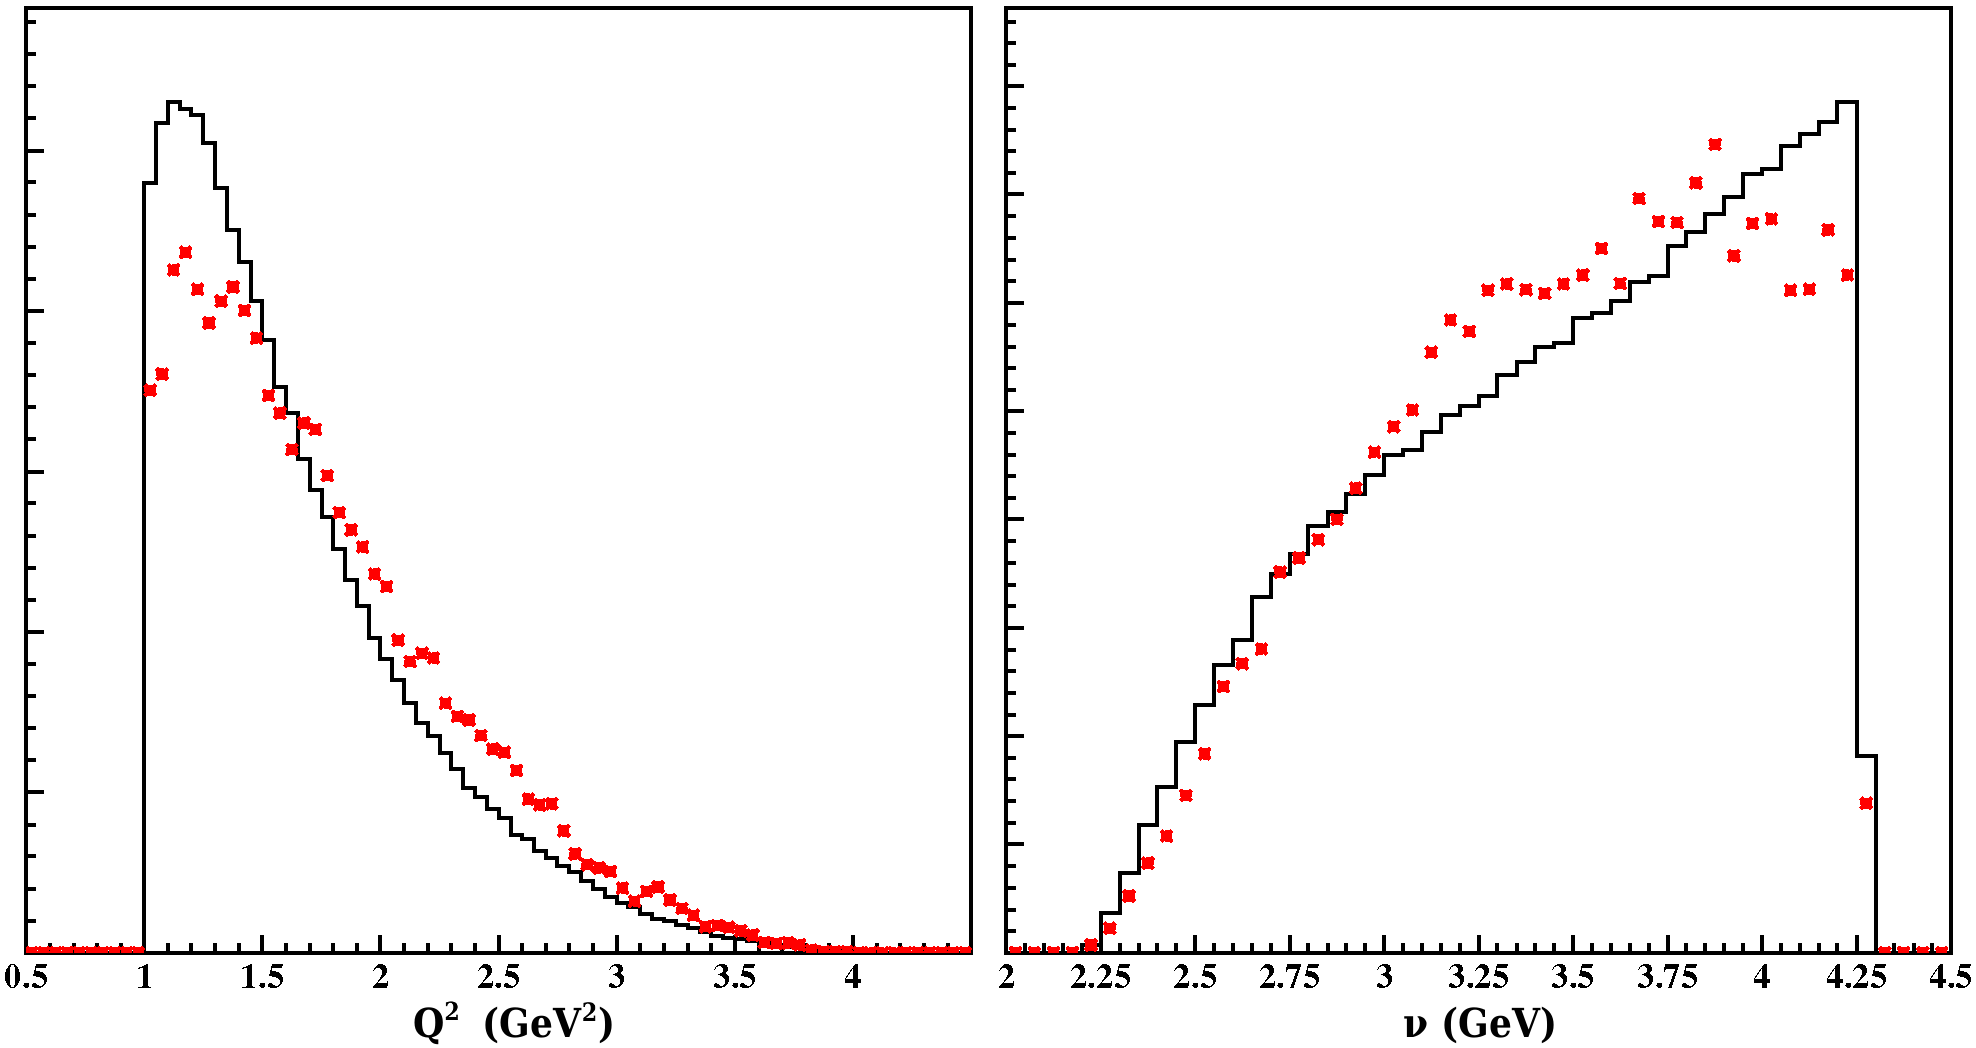
\includegraphics[width=12cm] {chap5-fig/El_compar.png}
\caption {Comparisons, for $Q^2$ (GeV$^2$/c$^2$) and $\nu$ (GeV), of the distributions
from simulated (red crosses) and experimental (histogram) data using deuterium target.}
\label{fig:compNuQ2}
\end{figure}

\begin{figure}[tbp]
\centering
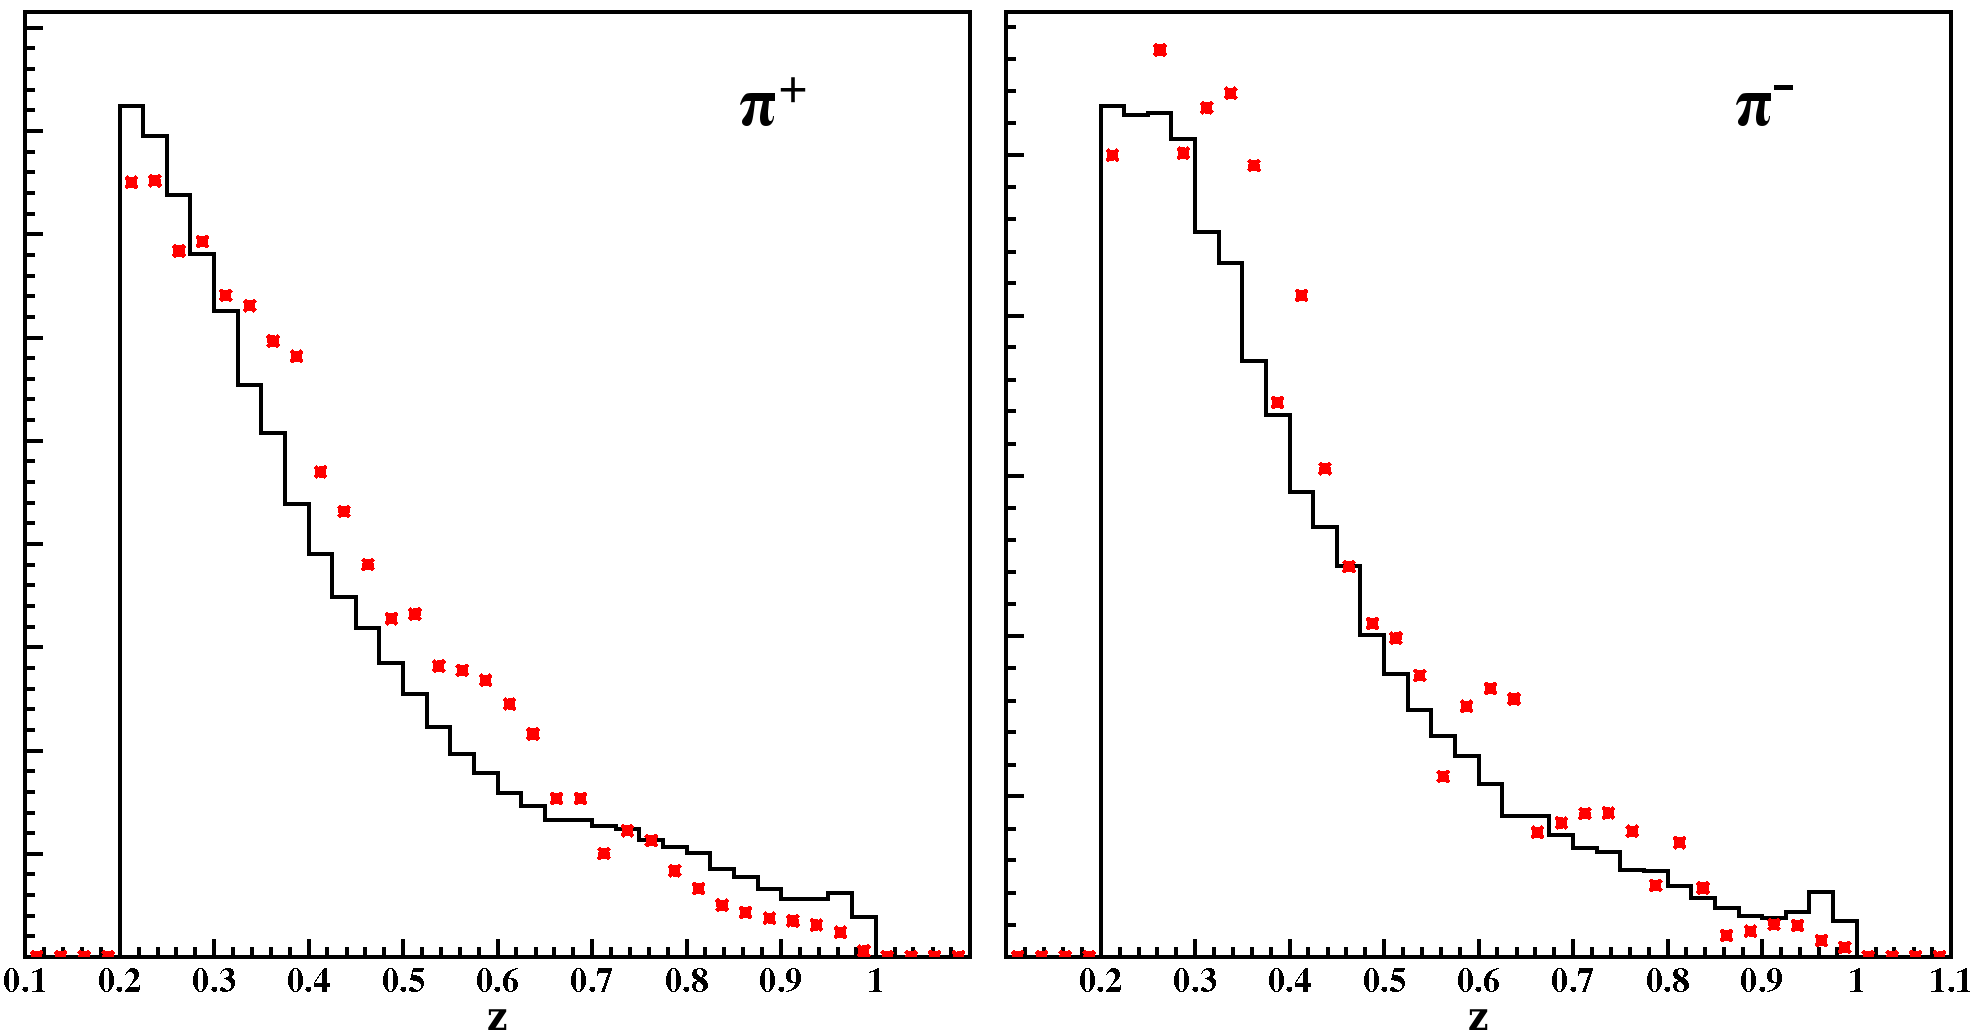
\includegraphics[width=12cm] {chap5-fig/z_compar.png}
\caption {Comparisons, for $z$ of charged pions, of the distributions
from simulated (red crosses) and experimental (histogram) data using deuterium target.}
\label{fig:compZ}
\end{figure}

\begin{figure}[tbp]
\centering
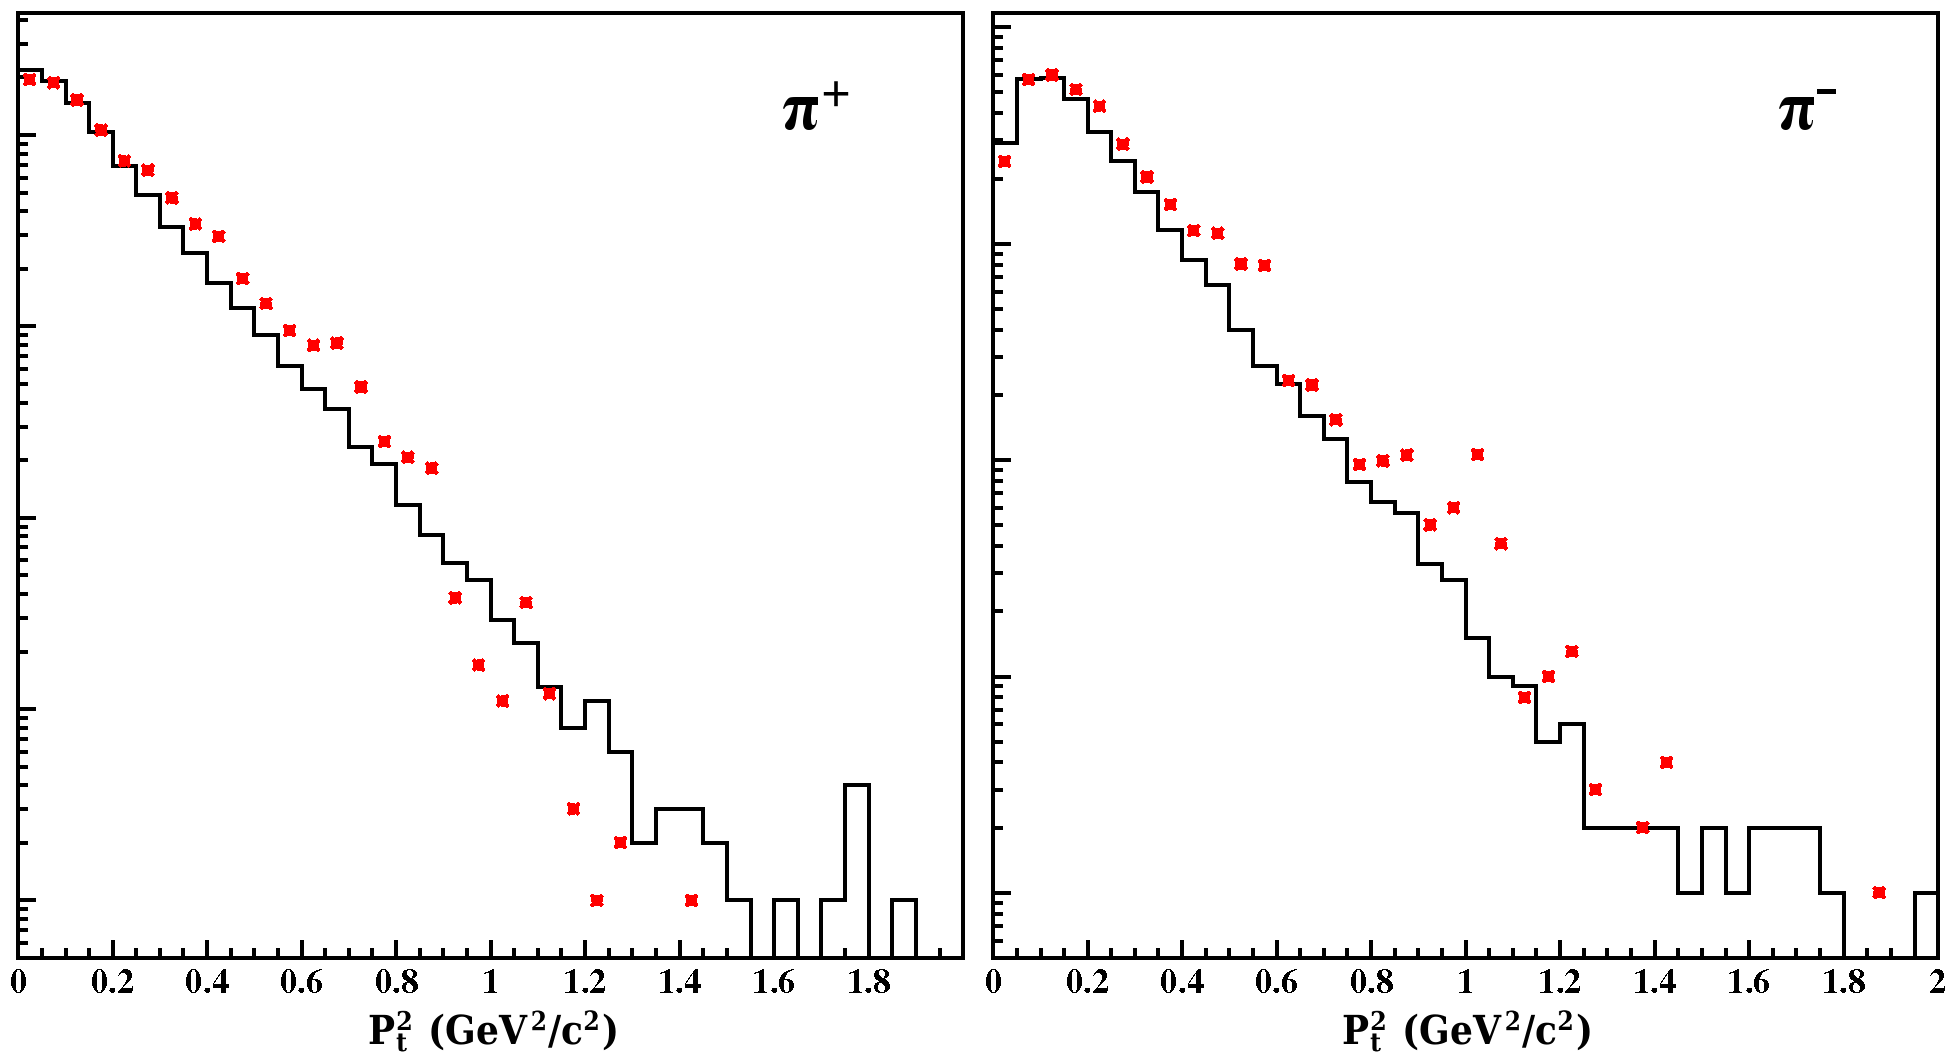
\includegraphics[width=12cm] {chap5-fig/pts_compar.png}
\caption {Comparisons, for \pt (GeV$^2$/c$^2$) of charged pions, of the distributions
from simulated (red crosses) and experimental (histogram) data using deuterium target.}
\label{fig:compPts}
\end{figure}

\begin{figure}[tbp]
\centering
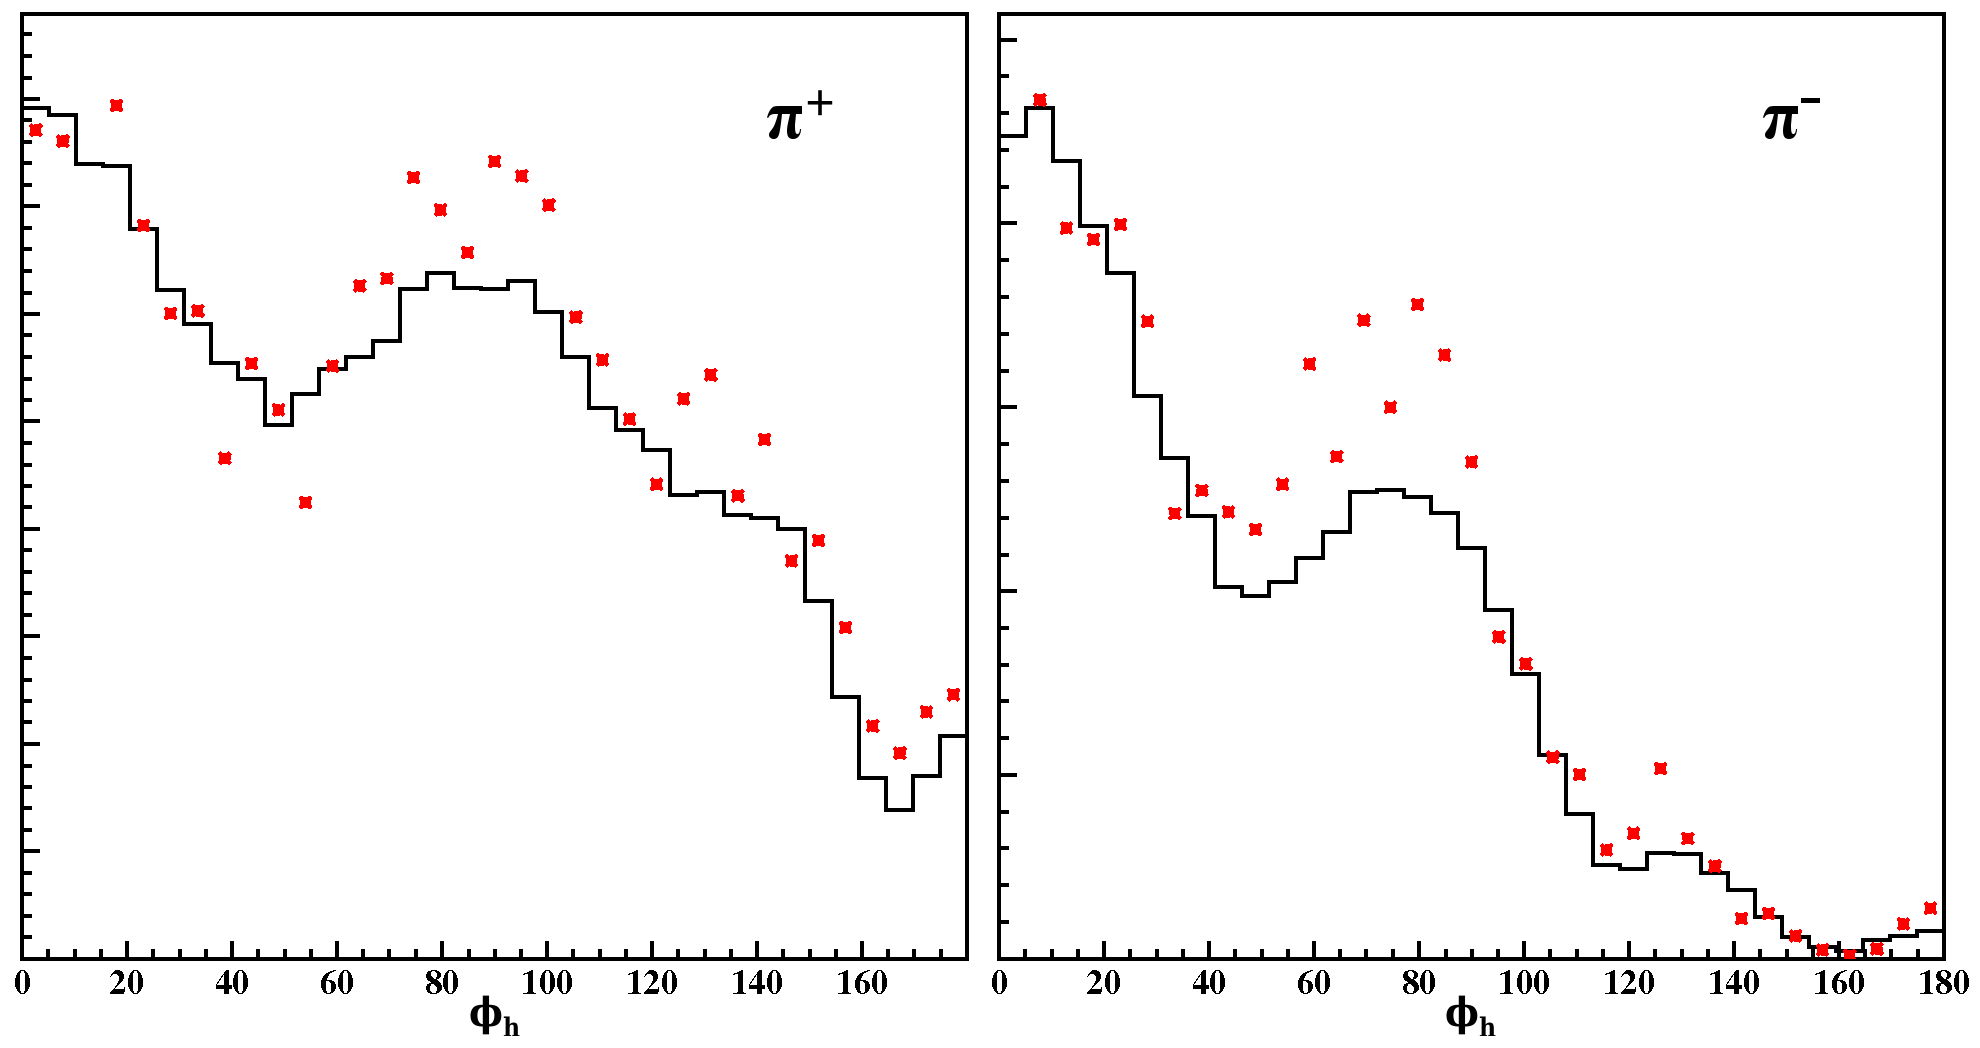
\includegraphics[width=12cm] {chap5-fig/phih_compar.png}
\caption {Comparisons, for $\phi_h$ of charged pions, of the distributions
from simulated (red crosses) and experimental (histogram) data using deuterium target.}
\label{fig:compPhih}
\end{figure}


\paragraph{Correction of the Data} ~\\
The acceptance correction coefficients are defined as the ratio of reconstructed and generated events,

\begin{equation}
\label{eq:acc}
\text{Acc} = {N_{rec} \over N_{gen}}.
\end{equation}

Experimental data were corrected using the weights defined as $\omega = 1/\text{Acc}$. These 
coefficients are calculated in many bins, in order to be independent of the imperfections of 
our event generator. However, an excess of bins could lead to a large bin 
migration\footnote{Fraction of events not reconstructed in the bin they were produced in.}, 
which introduces a bias in the evaluation of acceptance. Bin sizes are therefore chosen to
be larger than the resolution associated to each kinematic variable.

We used a 4-dimensional binning to divide the large phase space of our two particle final 
state. However, to evaluate systematic errors associated with this correction, we compared the
method using two different sets of kinematic variables, as presented in 
table~\ref{tab:AcceptBinning} and \ref{tab:AcceptBins}. The first set of variables is the one actually used for the
analysis and the second set is only used to evaluate the systematic errors, so in the 
following, the formulas are given only for the first set. The total number of bins is 
constrained by the amount of generated data and must be maintained reasonably low in order 
to keep a good statistical precision and a small bin migration.

\begin{table}[htbp]
  \centering
  \begin{tabular}{@{} cc @{}}
    \hline
    Variable & Number of bins \\ 
    \hline
    $\nu$    & 5 \\
    $x_{Bj}$ & 5 \\
    $p_h$    & 7 \\
    $t$      & 7 \\
    \hline
    Total    & 1225 \\
    \hline
  \end{tabular}
  \begin{tabular}{@{} c @{}}
  ~~~~~~\\
  ~~~~~~\\
  \end{tabular}
  \begin{tabular}{@{} cc @{}}
    \hline
    Variable & Number of bins \\ 
    \hline
    $Q^2$    & 5 \\
    $\nu$    & 5 \\
    $z_h$    & 7 \\
    $t$      & 7 \\
    \hline
    Total    & 1225 \\
    \hline
  \end{tabular}
  \caption{Variables and their associated number of bins used on the 
   multi-dimensional binning of our acceptance correction. The left panel 
   shows the variables used on this correction, and the right panel contains the 
   variables used on the evaluation of the related systematic uncertainties.}
  \label{tab:AcceptBinning}
\end{table}

\begin{table}[htbp]
\center
\begin{tabular} {|c|c|c|c|c|}
\hline
 $\nu$ & \xb & $p_\pi$ & $-t$ \\ \hline
 2.20 & 0.12 & 0.25 &-3.50 \\ 
 3.00 & 0.18 & 0.60 &-2.10 \\ 
 3.40 & 0.22 & 1.00 &-1.75 \\ 
 3.75 & 0.27 & 1.45 &-1.50 \\ 
 4.00 & 0.33 & 1.70 &-1.30 \\ 
 4.25 & 0.60 & 2.15 &-1.10 \\ 
      &      & 3.00 &-0.75 \\ 
      &      & 4.25 &-0.00 \\ \hline
\end{tabular}
\quad
\begin{tabular} {|c|c|c|c|c|}
\hline
 $Q^2$ & $\nu$ & $z$ & $-t$ \\ \hline
 1.00 & 2.20 & 0.00 & -3.50 \\
 1.20 & 3.00 & 0.20 & -2.10 \\
 1.40 & 3.40 & 0.40 & -1.75 \\
 1.65 & 3.75 & 0.45 & -1.50 \\
 2.10 & 4.00 & 0.52 & -1.30 \\
 4.00 & 4.25 & 0.62 & -1.10 \\
      &      & 0.80 & -0.75 \\
      &      & 1.00 & -0.00 \\ \hline
\end{tabular}
\caption{Bin limits used for the acceptance correction described in table \ref{tab:AcceptBinning}.}
  \label{tab:AcceptBins}
\end{table}

The weights ($\omega_{\pi^\pm}(\nu,x_{Bj},p_h,t)$) are extracted from 
the simulation using equation \ref{eq:acc}. However, these coefficients should not be applied to data before resolving the issues with bins that have either
\begin{itemize}
 \item too large weight values, i.e., very small acceptance, or
 \item very few reconstructed events and very large statistical errors, or
 \item a large fraction of events originally generated in another bin (bin migration issue).
\end{itemize}
To eliminate these bins we apply the following cuts:
\begin{equation} \label{eq:AccL1}
\left ({\delta \omega \over \omega}\right ) ^2 \times R_c \times \omega < 2,
\end{equation}
and
\begin{equation} \label{eq:AccL2}
N_{rec} > 4,
\end{equation}
where $\delta \omega / \omega$ is the relative error on the weight, and $R_c$ is the 
proportion of reconstructed events initially generated in an other kinematical bin. 
Figure~\ref{fig:AccCoef} shows $\omega$ distributions after applying these cuts. Around 
900 bins remain for both targets, but we noticed that these weights are much larger for 
$\pi^-$ compared to $\pi^+$, as an indication of a larger correction for the inbent 
particles. The motivation for using such a cut based on the product of different unrelated
values is actually directly linked to this problem. The $\pi^-$ acceptance drops very 
strongly at low \pt leading to very high weights, however there is no problem of bin migration
or low statistics because the generated yield is very high in this region. We found that 
the best way
to keep these bins while discarding bins where the weight might be slightly smaller but which 
have issues with bin migration and statistics was to apply this set of cuts.

In order to correct for these droped bins and reduce the sensitivity to the arbitrary in
the choice of the weights' cuts, we corrected the data with an additional two dimensional 
reweighting factor as:
\begin{equation}
\text{Acc}_2(\nu,p_h) = {\sum_{rec} \omega (\nu,x_{Bj},p_h,t)\over N_{gen}(\nu,p_h)}.
\end{equation}
where $\omega$ is the previously calculated weight or a 1 for a bin that was excluded by the 
cuts of equation \ref{eq:AccL1} and \ref{eq:AccL2}. One of the criteria for setting the limits 
in these equation is in fact to keep this reweighting factors, $\omega_2 = 1/\text{Acc}_2$, at 
the level of a few percents. This indicates that the previous method only missed a small 
fraction of the event in the first place and is a good indication of the sanity of the method.

\begin{figure}[tbp]
\centering
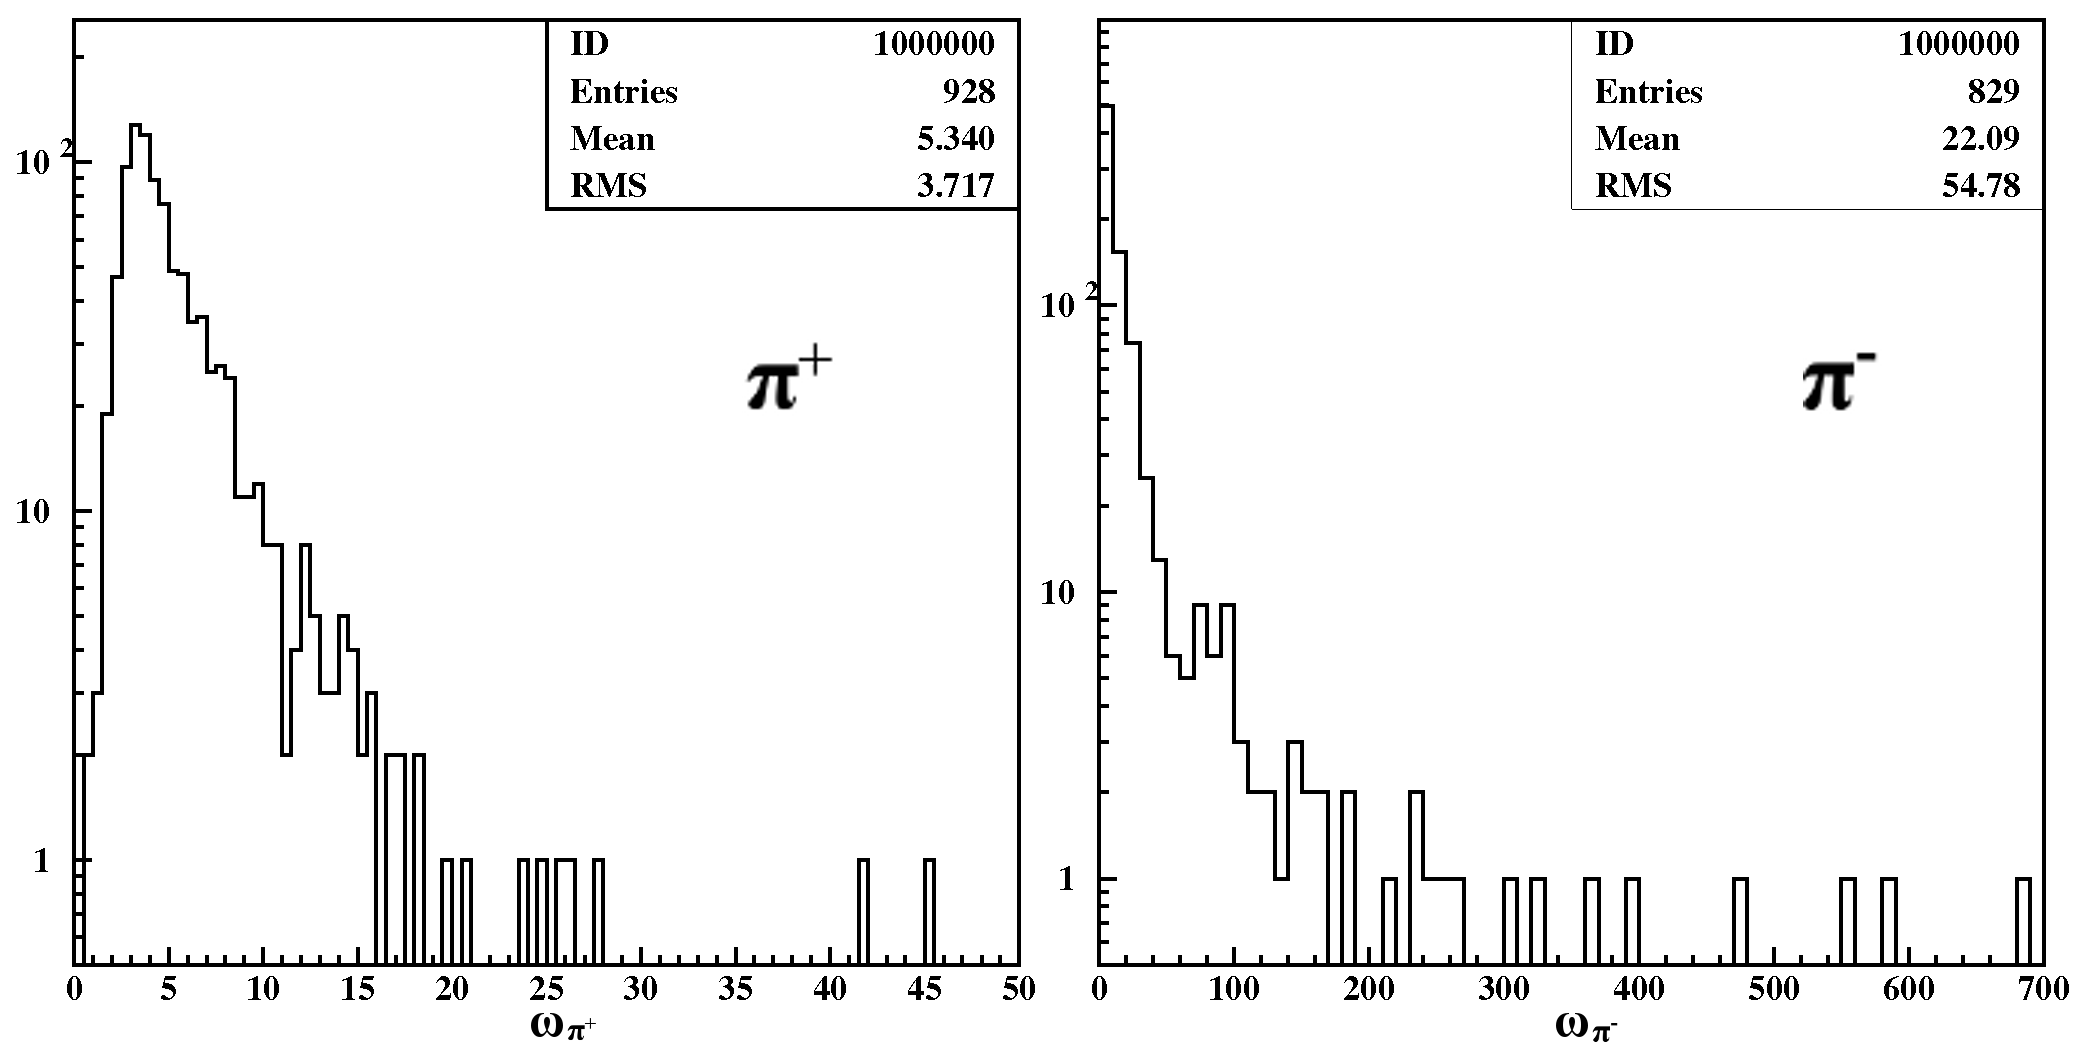
\includegraphics[width=14cm] {chap5-fig/pawpipdeut.png}
\caption {The extracted acceptance correction weights for pions on a deuterium target (not re-weighted).}
\label{fig:AccCoef}
\end{figure}

In order to correct the number of electrons in multiplicity ratios, we followed the semi-inclusive acceptance correction method by using only the two first dimensions ($\nu$ and $Q^2$). However, the reweighting was not used for electrons as all non-empty bins pass the two cuts, \ref{eq:AccL1} and \ref{eq:AccL2}.

\begin{figure}[tbp]
\centering
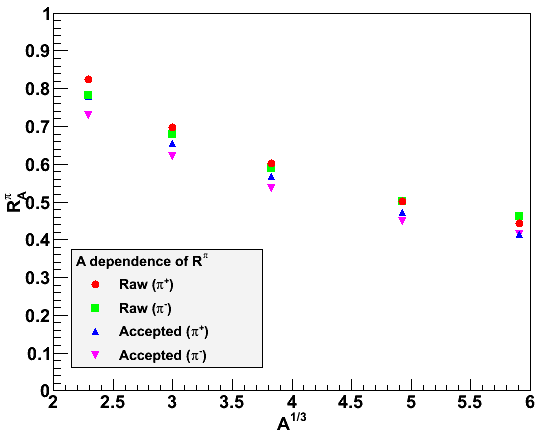
\includegraphics[width=7.4cm] {chap5-fig/b_RvA.png} 
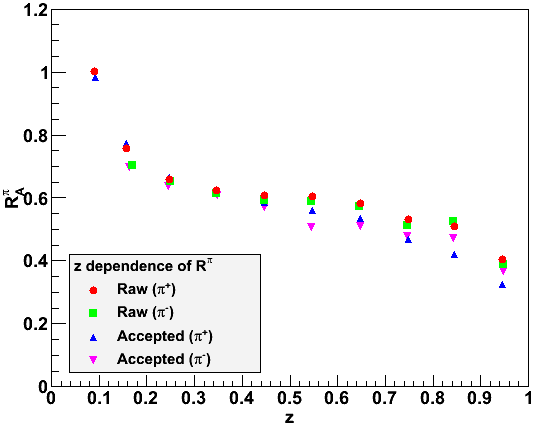
\includegraphics[width=7.4cm] {chap5-fig/b_RvZ.png} 
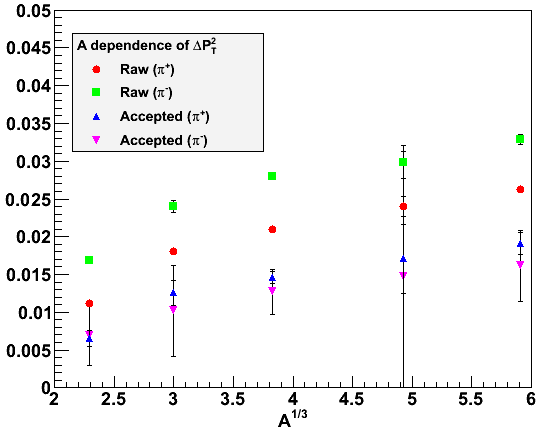
\includegraphics[width=7.4cm] {chap5-fig/b_PvA.png} 
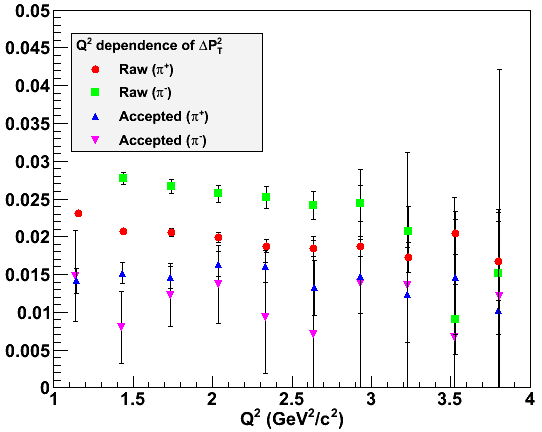
\includegraphics[width=7.4cm] {chap5-fig/b_PvQ2.png} 
\caption {Preliminary results are compared with the acceptance corrected ones, 
for multiplicity ratios (top) and transverse momentum broadening 
(bottom). Only statistical errors are shown.}
\label{fig:AcceptPlots}
\end{figure}

Figure \ref{fig:AcceptPlots}, where only statistical errors are 
represented, shows the new results after applying the acceptance correction.
The acceptance correction effects appear to be in the order of $10$\% for 
multiplicity ratios and $30$\% for the transverse momentum broadening. This is a surprisingly significant correction with regard to a few centimeters separating the two targets. The reason for such a large correction is that the small shift in the $z$-vertex position changes slightly the minimum angle of the detector in the region where most hadron production is concentrated, {\it i.e.} at low \pt close to the beam line. The $\pi^-$s were more affected due to the inbending magnetic field. Indeed, the low \pt $\pi^-$s had very low acceptance which led to large correction factors. The large spread in weights makes the errors on \dpt very large, and the related results difficult to exploit. However, our transverse momentum broadening 
results of both pions matched each other after this correction, which is similar 
to the HERMES results (see figure~\ref{fig:her3}).

\subsubsection{Coulomb Correction}
\label{CCor}

The large electric charge of our nuclear targets create an electric field that 
should be taken into account at our energies. Besides the fact that the nuclear 
electric field accelerates or decelerates the incoming and outgoing charged 
particles, it has some non trivial effects such as the focusing of low energy 
particles. Aste {\it et al.}~\cite{Aste:2005wc} showed that these Coulomb 
effects could be corrected for by using an effective momentum approximation at 
large momenta ({\it i.e.}, $Q^2>.5$ GeV$^2$). As our kinematics coverage is 
beyond this limit, we decided to use this approximation on the Coulomb 
correction of our data-sets. According to Aste {\it et al.}, the best effective 
potential approximation is given by $\bar V= 0.8 V_0$, where $V_0$ is the 
electrostatic potential at the center of nuclei. The latter is evaluated as 
$V_0= -3 \alpha_{EM} Z / (2 R)$, where $\alpha_{EM}$ is the fine-structure 
constant, $Z$ is the proton number, and $R$ is the radius of the nuclei. Table 
\ref{tab:Coulomb} contains the used values of $V_0$ and $\bar V$ on different 
nuclear target's analysis. The Coulomb correction is applied to both electrons 
and charged pions before calculating the plotted kinematical variables.

\begin{table}[htbp]
  \centering
  \begin{tabular}{@{} ccc @{}}
    \hline 
Nucleus & $V_0$ (MeV)  &  $\bar V$ (MeV) \\ \hline
$^2$H & -1 &   -1 \\
C   &  -4 &    -3 \\
Al  &  -7 &    -6 \\
Fe  & -11 &    -9 \\
Sn  & -17 &   -14 \\
Pb  & -23 &   -19 \\
    \hline
  \end{tabular}
  \caption{The $V_0$ and $\bar V$ values used on Coulomb corrections for different charged particles.}
  \label{tab:Coulomb}
\end{table}

TODO Add figures of the effect and comment from review answers!

\subsubsection{Radiative Correction}
\label{RadCor}

The QED diagrams shown in figure \ref{fig:FDRadCorr} contribute to the measurement
of the leptoproduction of hadrons. The diagram (a) is the Born cross section, the
others are radiative contributions that we would like to subtract in order to 
have results more easily interpretable in term of hadronic physics.
This substraction is what we call the radiative correction, as can be seen 
this correction should take care of real photon productions (diagrams b and c)
but also virtual photon exchange (diagram d) and photon self energy (diagram e).
We neglect exchanges of photons with hadrons as they are suppressed due to the 
large mass of hadrons in comparison to electrons. For practical reasons, we also 
limit this correction to leading order as can be seen from the presented diagrams.

\begin{figure}[htp]
\centering
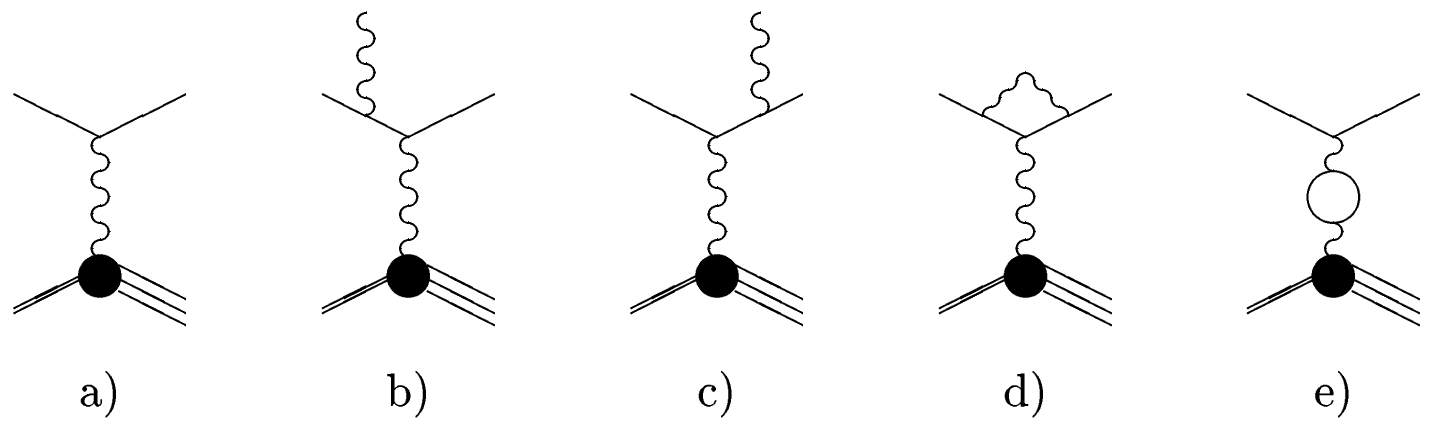
\includegraphics[width=12cm] {chap5-fig/RadDiag.png}
\caption {Diagrams taken into account in the HAPRAD 2 code \cite{Akushevich:2007jc}. The 
diagrams b to e contribute to the first order calculation of the radiative 
effects of the Born cross section represented in diagram a.}
\label{fig:FDRadCorr}
\end{figure}

The radiative correction is not expected to be important in the multiplicity 
ratios due to the double cancellation between the different contributions of 
the ratio. However, its impact on the transverse momentum brodening is more 
difficult to anticipate. We therefore decided to calculate the correction using 
the recent Haprad 2 code \cite{Akushevich:2007jc} with adaptations to include
nuclear effects such as Fermi motion \cite{Osipenko:PC}. This calculation is
using modeled semi-inclusive structure functions (based on former CLAS
data \cite{Akushevich:2007jc}) and modeled exclusive channels from MAID 2003
\cite{Drechsel:1998hk}. This calculation is the state of the art in the matter
as it is an exact calculation in the complete five dimension cross section
and do not use the peaking approximation generally used in previous method.

To apply the radiative correction, we apply a weight to each events in a fashion
similar to the acceptance correction. The HAPRAD 2 code provides 
$\delta = \sigma_{obs} / \sigma_B$ at given kinematics. Table \ref{tab:RCBins} 
shows the binning used to calculate the radiative correction weights.
We chose to make a finer 
binning for the radiative corrections than for acceptance as the computing time 
to calculate weights is more reasonnable (around 1000 days of cpu time). 

\begin{table}[htbp]
\center
\begin{tabular} {|c|c|c|c|c|c|c|}
\hline
Bin Nb & $\nu$ & \xb & $p_\pi$ & $-t$ & $\phi$ \\ \hline

 0     & 2.25 & 0.12 & 0.20 & -3.50 &   0.0 \\ 
 1     & 2.45 & 0.15 & 0.35 & -2.10 &  18.0 \\ 
 2     & 2.66 & 0.17 & 0.50 & -1.75 &  36.0 \\ 
 3     & 2.82 & 0.18 & 0.75 & -1.50 &  54.0 \\ 
 4     & 2.96 & 0.19 & 1.00 & -1.30 &  72.0 \\ 
 5     & 3.07 & 0.20 & 1.60 & -1.10 &  90.0 \\ 
 6     & 3.17 & 0.21 & 2.20 & -0.75 & 108.0 \\ 
 7     & 3.27 & 0.22 & 4.25 &  0.00 & 126.0 \\ 
 8     & 3.37 & 0.23 &      &       & 144.0 \\ 
 9     & 3.46 & 0.24 &      &       & 162.0 \\ 
10     & 3.55 & 0.25 &      &       & 180.0 \\ 
11     & 3.64 & 0.26 &      &       &       \\ 
12     & 3.72 & 0.27 &      &       &       \\ 
13     & 3.80 & 0.28 &      &       &       \\ 
14     & 3.87 & 0.30 &      &       &       \\ 
15     & 3.94 & 0.33 &      &       &       \\ 
16     & 4.01 & 0.36 &      &       &       \\ 
17     & 4.07 & 0.39 &      &       &       \\ 
18     & 4.12 & 0.43 &      &       &       \\ 
19     & 4.18 & 0.48 &      &       &       \\ 
20     & 4.25 & 0.56 &      &       &       \\   
                                          
\hline
\end{tabular}
\caption{Bin limits used for the radiative correction described in section \ref{RadCor}.}
  \label{tab:RCBins}
\end{table}

We show in figure \ref{fig:RCexample} a selected sample of radiative correction factors
($= \delta_{Fe} / \delta_D$) in order to illustrate the expected effect on observables.
In the large majority of the cases the factors are within 5\% of 1, so we do not expect to
see a strong effect on the final results where these will be integrated. This is confirmed 
in figure \ref{} ... In the case of the transverse momentum braodening, the variations
appear to ...

\begin{figure}[tbp]
\centering
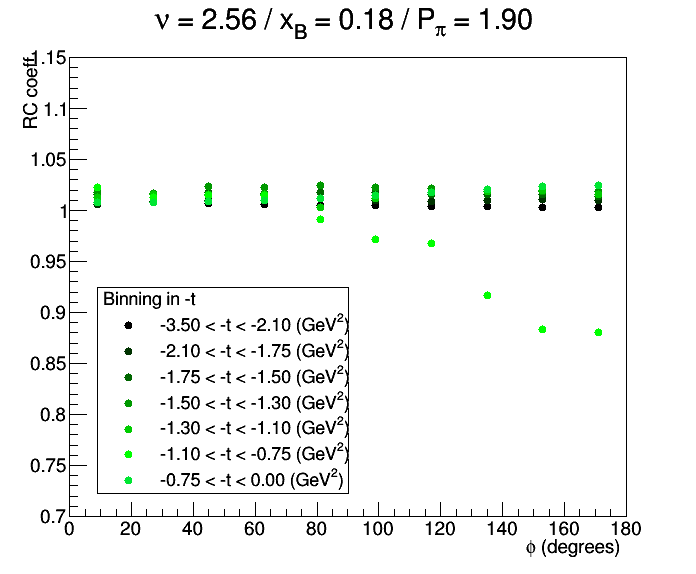
\includegraphics[width=7cm] {chap5-fig/ElecRadWei_Iron_2356.png}
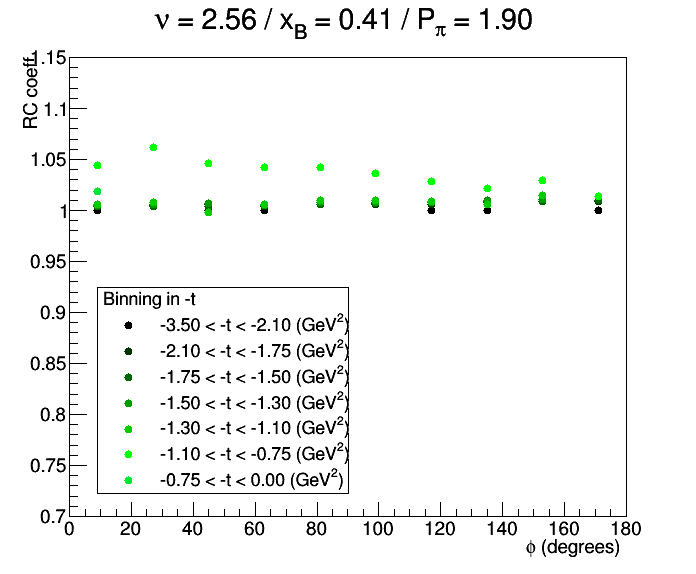
\includegraphics[width=7cm] {chap5-fig/ElecRadWei_Iron_3756.png}
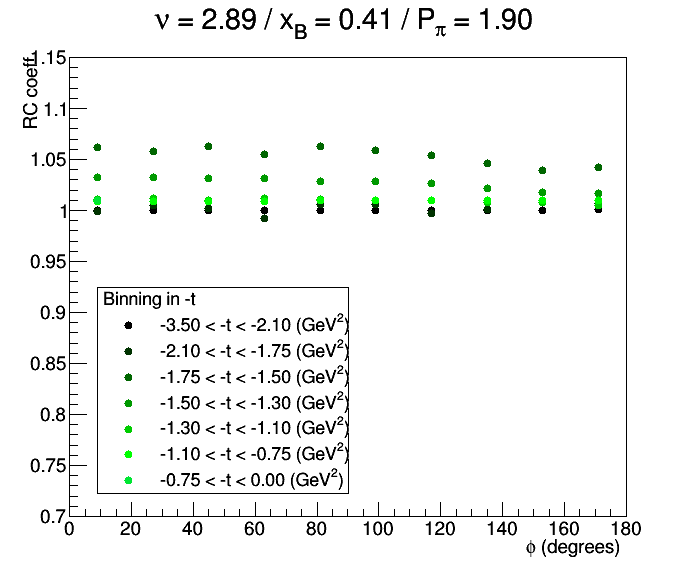
\includegraphics[width=7cm] {chap5-fig/ElecRadWei_Iron_7756.png}
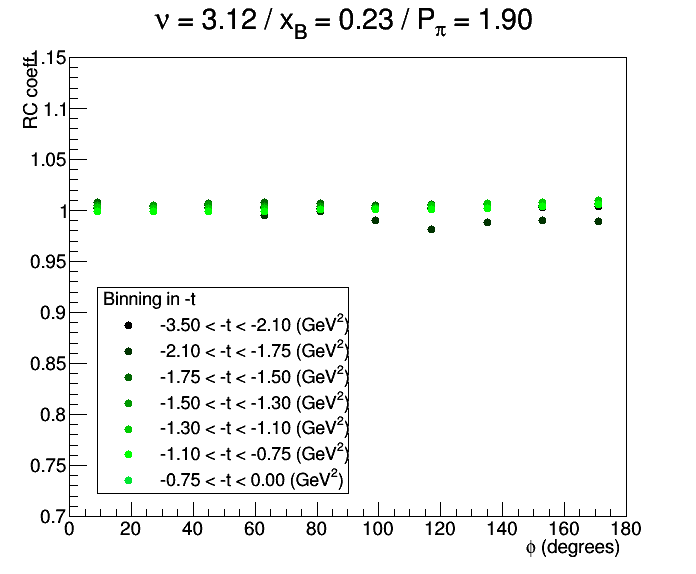
\includegraphics[width=7cm] {chap5-fig/ElecRadWei_Iron_10756.png}
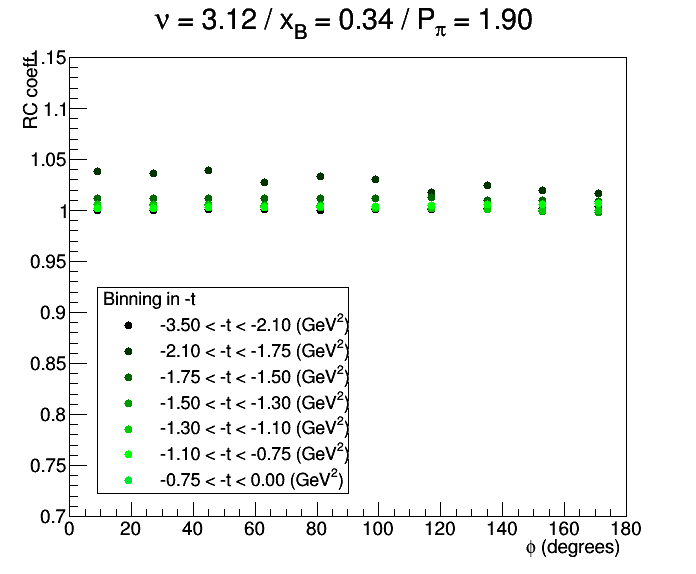
\includegraphics[width=7cm] {chap5-fig/ElecRadWei_Iron_11556.png}
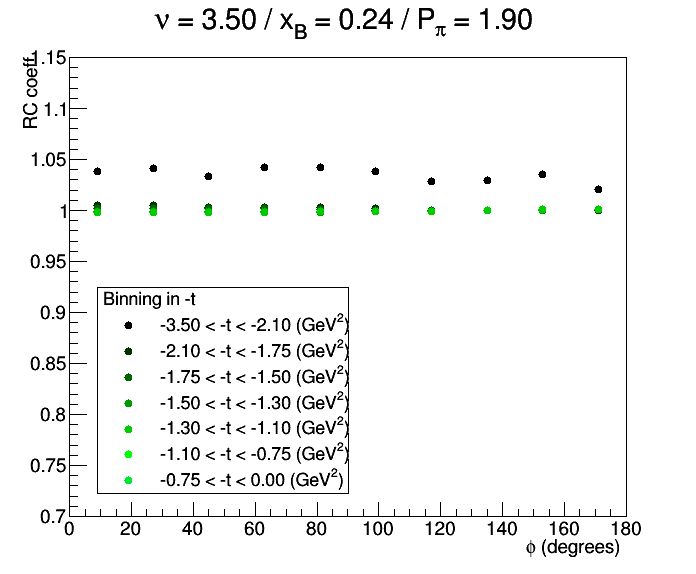
\includegraphics[width=7cm] {chap5-fig/ElecRadWei_Iron_18956.png}
\caption {RC factors ($= \delta_{Fe} / \delta_D$) as a function of $\phi$ and 
$-t$ for a selection of bins specified above each figure.}
\label{fig:IsoSpin}
\end{figure}

\begin{figure}[tbp]
\centering
\caption {Preliminary results ..., 
for multiplicity ratios (top) and transverse momentum broadening 
(bottom). Only statistical errors are shown.}
\label{fig:RCPlots}
\end{figure}

\subsubsection{Isospin Correction}

The important excess of neutrons in heavy nuclei leads to a modification of 
both $\pi$ multiplicities regardless of nuclear effects. Using Hall~C results 
\cite{Asaturyan:2011mq}, shown in figure \ref{fig:IsoSpin}, we evaluated the 
correction factors for the imbalance of u/d quarks in heavy nuclei compared
to deuterium. Our simple estimation is solely based on proton and neutron 
numbers and assumes that this isospin correction does not depend on any
kinematic variable. We found that multiplicity ratios of $\pi^+$ need small
corrections, shown in table~\ref{tab:isospin}. The effect on $\pi^-$s was 
found to be consistent with zero, so no correction was applied to their 
multiplicity ratios. We attribute a normalization error to the finale results
equal to 10\% of the isospin correction. This is evaluated based on the 
precision of the Hall~C measurement.

\begin{figure}[tbp]
\centering
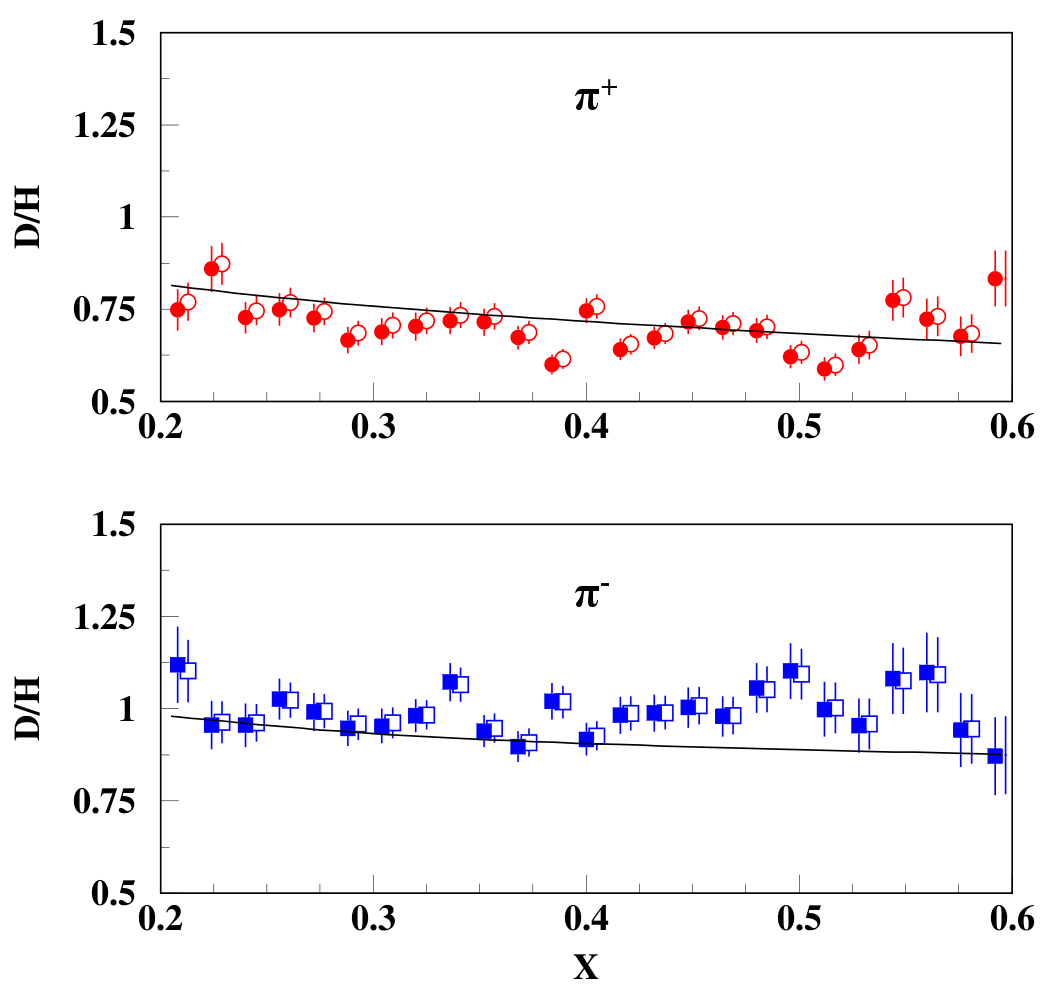
\includegraphics[width=10cm] {chap5-fig/HallC-Isospin.png}
\caption {Ratios of deuteron over proton for $\pi^+$s and $\pi^-$s 
as a function of \xb at $z=0.55$ \cite{Asaturyan:2011mq}.}
\label{fig:RCexample}
\end{figure}

\begin{table}[htbp]
  \centering
  \begin{tabular}{@{} cc @{}}
    \hline
    Target & Isospin  \\ 
           & correction \\ 
    \hline
    C & 0 \\
    Al & 1.5\%\\
    Fe &  3\% \\
    Sn &  8\%\\
    Pb &  10\% \\
    \hline
  \end{tabular}
  \caption{Isospin correction applied to $\pi^+$ multiplicity ratios for different targets.}
  \label{tab:isospin}
\end{table}

It is important to mention that the isospin correction is only relevant to 
rate measurements. The transverse momentum broadening could, in principle, 
be affected, however, the results from \cite{Asaturyan:2011mq} showed no 
isospin effects in \ptp. Therefore, we are confident that our \dpt results 
should not be sensitive to any isospin effects.

We finally note that the $A$ dependence of multiplicity ratios of both 
charged pions became parallel after the isospin correction\footnote{Within 
normalization errors presented in section \ref{sec:TotSys}} (see figure 
\ref{fig:IsoPlot}). Considering previous measurements and existing models, 
this result was expected and demonstrates the importance of this correction.

\begin{figure}[tbp]
\centering
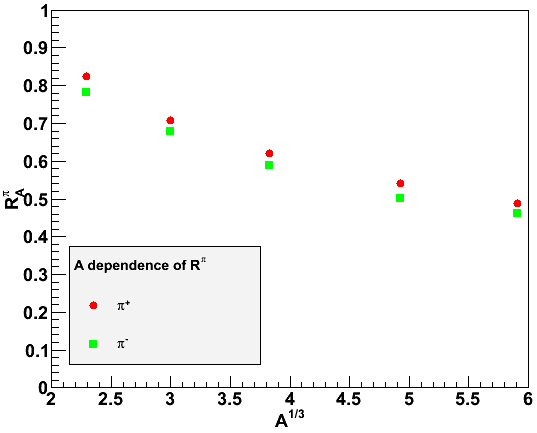
\includegraphics[width=8.5cm] {chap5-fig/c_RvA.png}
\caption {Multiplicity ratios as a function of $A^{1/3}$ with the isospin correction applied.}
\label{fig:IsoPlot}
\end{figure}

\subsubsection{Endcap correction}

TO BE IMPLEMENTED IN THE ANALYSIS

The goal of this work is to correct the measured multiplicity ratio:
\begin{equation}
  R_h^A |_{corr} = {N_h^A / N_e^A \over (N_h^D-N_h^{EC}) / (N_e^D-N_e^{EC})},
\end{equation}
with the $EC$ target being the endcaps of the liquid target. Using a Taylor expension at first order for small $N^{EC}$, we find that:
\begin{equation}
  {N_h^D-N_h^{EC} \over N_e^D-N_e^{EC}} = {N_h^D \over N_e^D} - {N_h^{EC} \over N_e^D} + {N_e^{EC} N_h^D \over {N_e^D}^2}.
\end{equation}
After few straightforward transformation, we get
\begin{equation}
  R_h^A |_{corr} = R_h^A \left( 1 - {N_e^{EC} \over N_e^D} \left( 1-R_h^{Al} \right) \right).
\end{equation}
Based on target thickness ${N_e^{EC} \over N_e^D} \sim 0.03$ and $R_h^{Al} \sim 0.65$, the correction is on average a 1\% decrease of the measured multiplicity ratio.

With the same method, the transverse momentum broadening can be corrected with:
\begin{equation}
  \Delta P_T^2 |_{corr} = \Delta P_T^2 + R_h^{Al} {N_e^{EC} \over N_e^D} \Delta P_T^2|_{Al}
\end{equation}


\subsection{Systematic Uncertainties}
\label{sec:TotSys}

In this section, we are presenting details of our two types of systematic uncertainties. The point-to-point systematic errors, that vary with kinematical variables, were calculated bin by bin for each result. They are caused by uncertainties on the particles' identification cuts and the CLAS acceptance. The normalization errors are attributed globally since they don't depend on kinematics. They are due to acceptance effects, target's misidentification, and the isospin correction.

\subsubsection{Quality of the Detection}
\label{SysId}

The simulation of the CLAS detector, using the GSIM package, is used 
to evaluate the systematic errors correlated with:

  - experimental resolution of kinematical variables,

  - particles' misidentification,

  - particles' scattering in different detectors,

  - particles' energy loss.\\


To evaluate these errors, we are comparing the kinematics of reconstructed 
particles with the generated ones. Each reconstructed particle is associated 
with its generated parent if both particles have a similar momentum and 
angle. The precision of the measured kinematical distribution 
$\Delta p$, $\Delta \theta$ and $\Delta \phi$ were determined as $\Delta x = 
{\sum_n |x_{gen} - x_{rec}| \over n}$. Using the same simulation as for 
the acceptance, we found 
${\delta p \over p } = 0.03$, $\delta \theta = 3$ mrad and $\delta \phi = 
10$~mrad. While being larger than the nominal CLAS resolutions published in 
\cite{Mecking:2003zu}, they are still reasonable for our measurement. We also 
evaluated these errors in term of other variables, such as 
$\delta Q^2 \sim 0.013$ GeV$^2$/c$^2$, $\delta z \sim 0.4 \%$ and $\delta 
P_\perp^2 \sim 0.004$ GeV$^2$/c$^2$ (\footnote{These values are evaluated for 
a typical kinematics range. The results can be larger at extreme kinematics 
(large \pt or Q$^2$).}). These errors are overall negligible since they are 
several times smaller than our usual bin sizes (see figures in a section 
\ref{prelim}). 

We also evaluated the particles' misidentification and scattering on materials
from the detectors or coils. For this study, we are looking at reconstructed 
particles that do not have a clear parent (either because they are misidentified
or because they scattered and their kinematic changed significantly). The 
misidentification of electrons was found to be small, of the order of 1 in 
1000 $e^-$ in all the kinematic space, hence this issue does not contribute 
significantly to this uncertainty. We found however for pions
a high proportion of accidental events on the kinematical distributions tails, 
in particular of the \pt distribution. This effect is due to the low 
probability to produce high \pt events, leading to an increased relative 
contribution from the accidental background. As a consequence, we used the 
following cut $p_\perp^2 < 1.5$~GeV$^2$/c$^2$, which discards only a very 
little amount of data (about 1 in 30000 $\pi$). On the contamination side,
most events come from kaons with momenta above 2~GeV/c ($\sim$ 3\% for 
$\pi^+$s and $\sim$ 0.5\% for $\pi^-$s). Protons also contaminate the 
$\pi^+$ sample but only for the highest momenta (up to a few \%). 

In conclusion, the uncertainty related to particles' misidentification is 
taken into account with the attribution of a point-to-point systematic 
error equal to 100\% of the contamination level. The accidentals are taken 
care of using a cut on the high \pt distribution. Finally, resolution effects
were found to be negligible.

\subsubsection{Target Reconstruction}

Because of reconstruction errors or scattering on detector material, it 
is possible to associate a particle with the wrong target. To estimate this 
effect, we looked, in the experimental data, at the number of reconstructed 
events upstream and downstream of our targets, where nothing should be 
detected. Thus, we defined two test regions (see figure \ref{fig:targetleak}) 
to evaluate the associated contamination between the targets. The upstream 
region, named test region 1, is of the size of the solid target's selection 
cut to evaluate the contamination from the liquid target. The downstream region, 
named test region 2, covers the same size of the liquid target's selection cut 
to estimate the leak from the solid target. The distance between detection and 
test regions is identical to the distance between the two targets' detection 
regions. 

We found that the number of electrons in the test region 1 and 2 represents, 
respectively, 1 and 2\% of the total number of events. However, in the case 
of semi-inclusive measurements, where we request two particles coming from the
same spot in the final state, this number drastically dropped to $\sim$0.01\%. 
Therefore, only the number of electrons is significantly affected by the 
target's contamination issue, which is an issue only for multiplicity ratios.
We associate a normalization error of 1\% to all multiplicity ratios to account
with this issue.

\begin{figure}[tbp]
\centering
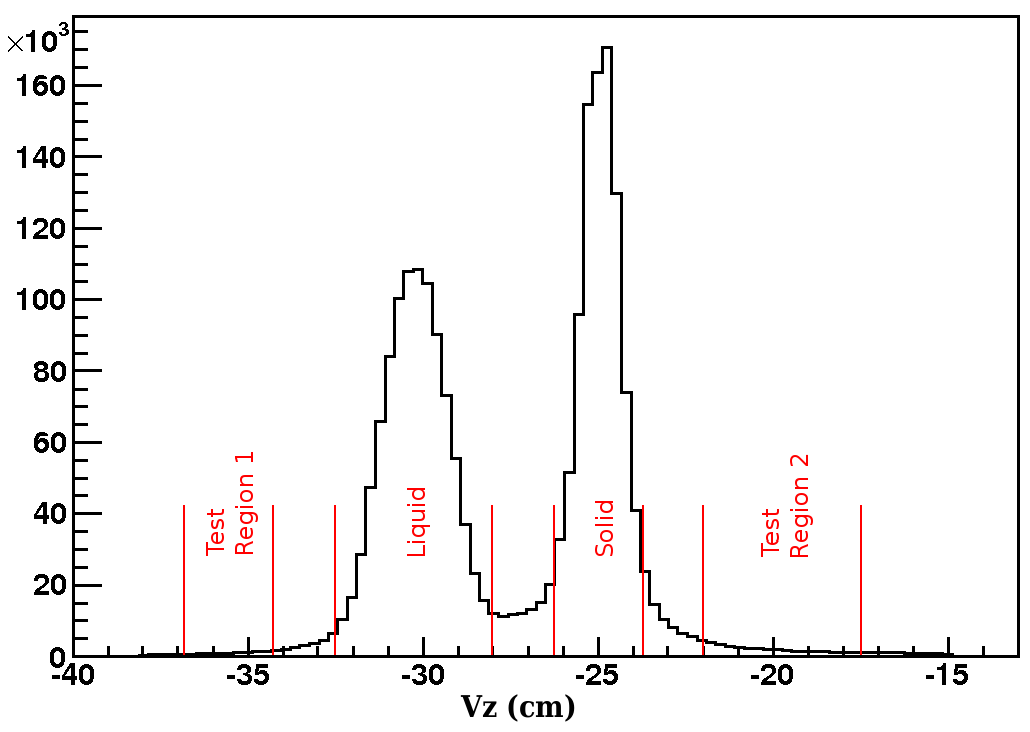
\includegraphics[width=9cm] {chap5-fig/Vertex.png}
\caption {Vertex distribution along a z direction (in cm), i.e. along the 
beam line. In red are shown the cuts used to evaluate the leak from one target to 
another.}
\label{fig:targetleak}
\end{figure}

\subsubsection{Acceptance}

After testing several different acceptance correction methods, we finally 
converged with the one using four dimensions and a limited number of bins.
The two different approaches to binning the data presented on a table 
\ref{tab:AcceptBinning} are used to evaluate the systematic errors. The 
difference between these two methods on iron data are used to evaluate 
the relative uncertainties presented in a table~\ref{tab:SysAcc}. We noticed 
the significantly large errors for $\pi^-$s, which were expected, due to their 
larger acceptance weights. Systematic errors are also
considerably larger for \dpt measurements. This is mainly due to the nature of 
the \dpt observable; as it is a difference, it enhances relative errors 
rather than cancelling them. 

\begin{table}[htbp]
  \centering
\renewcommand{\arraystretch}{1.3}
  \begin{tabular}{|c|c|c|}
    \hline
    Variable & Normalization & Point to point \\ 
             & errors        & errors         \\ 
    \hline
    $R^{\pi^+}_A$  & 1.2\% & 1.5\%  \\
    $R^{\pi^-}_A$  & 2.5\% & 2.6\%   \\
    $\langle \Delta P_\perp^2 \rangle^{\pi^+}_A$ & 5\% & 11\% \\
    $\langle \Delta P_\perp^2 \rangle^{\pi^-}_A$ & 5\% & 21\% \\
    \hline
  \end{tabular}
  \caption{Relative errors on pions' observables using the two weighting 
           methods described in the text.}
  \label{tab:SysAcc}
\end{table}

\subsubsection{Total Systematic Budget}

The point-to-point errors include contributions from particle 
misidentifications and acceptance effects. The normalization error, which is 
independent of kinematic variables, are due to acceptance effects, target 
misidentification and the isospin correction. The various constributions 
to the systematic normalization error are summarized in table~\ref{tab:sysid}. 

\begin{table}[htbp]
  \centering
\renewcommand{\arraystretch}{1.3}
  \begin{tabular}{|c|cc|cc|}
    \hline
              & $R_A^{\pi^+}$  & $R_A^{\pi^-}$ & \dptp$^{\pi^+}$ &  \dptp$^{\pi^-}$\\ 
    \hline
    Acceptance & 1.2\% & 2.5\% & 5\% & 5\% \\
    Target id. & 1\% & 1\% & 1\% & 1\% \\
    Isospin (Pb)& 1\% & 1\% & 1\% & 1\% \\
    Total      & 1.9\% & 2.9\% & 5.2\% & 5.2\% \\
    \hline
  \end{tabular}
  \caption{Total normalization uncertainties for both charged pions.}
  \label{tab:sysid}
\end{table}


\subsection{Cross Checks}
\label{sec:XChecks}

The goal here is to check known results in order to make sure we have normalization right. This is 
especially important since discrepencies with Hayk's analysis have been found and demonstrated the 
normalization to be a tricky problem.

\subsubsection{Inclusive electron normalization}

We expect the EMC ratio to cross unity around 0.3 - 0.35 and we know precisely the target thickesses.
From these we check our inclusive normalization...

\subsubsection{Pion ratio from Hall-C}

In paper from Hall-C they present results shown in fig 20 (to reproduce here). The bin corresponds to 
1.5 < Q2 < 4 GeV2, 0.35 < xb < 0.45, 0.5 < z < 0.6 and Pt2 < 0.2. They find ratios of 0.556+-0.011 for pi+
and 0.520+-0.011 for pi-. Note that it is not a double ratio and should be affected by the EMC effect,
moreover they do not make an isospin correction which is 1.5\%.

Put my result here
